\documentclass[10pt,twocolumn]{article}

\usepackage[margin=0.68in]{geometry}
\usepackage{amsmath}
\usepackage{booktabs}
\usepackage{xcolor}
\usepackage{listings}
\usepackage{graphicx}
\usepackage{tikz}
\usepackage{array}
\usepackage{float}
\usepackage{url}
\usepackage{xspace}
\usepackage{hyperref}

\usetikzlibrary{arrows.meta,positioning,fit,shapes.geometric}
\setlength{\columnsep}{0.24in}
\setlength{\emergencystretch}{2em}
\setcounter{topnumber}{3}
\setcounter{dbltopnumber}{3}
\renewcommand{\topfraction}{0.95}
\renewcommand{\dbltopfraction}{0.95}
\renewcommand{\textfraction}{0.05}
\renewcommand{\floatpagefraction}{0.80}
\renewcommand{\dblfloatpagefraction}{0.80}


\hypersetup{
  colorlinks=true,
  linkcolor=blue!55!black,
  citecolor=blue!55!black,
  urlcolor=blue!55!black,
  pdftitle={When Should an Agent Write a Program? Cost and Context of Code-Mode Tool Calling},
  pdfauthor={Mehmet Öner Yalçın},
  pdfsubject={A production-client measurement study of native MCP orchestration and Toolplane-mediated execution}
}
\newcommand{\toolplane}{\textsc{Toolplane}\xspace}
\newcommand{\direct}{\textsc{Direct}\xspace}
\newcommand{\codemode}{\textsc{Code}\xspace}
\newcommand{\usd}[1]{\$#1}
\newcommand{\finding}[1]{\paragraph{Finding.} \emph{#1}}
\setlength{\abovecaptionskip}{4pt}
\setlength{\belowcaptionskip}{5pt}
\tikzset{
  flowarrow/.style={-{Latex[length=2.2mm]}, thick, draw=gray!75!black},
  faintarrow/.style={-{Latex[length=2.0mm]}, thick, dashed, draw=gray!65!black},
  surfacebox/.style={draw=purple!60!black, fill=purple!7, rounded corners=2pt,
    align=center, inner sep=5pt, minimum height=8mm, font=\small},
  nativebox/.style={draw=teal!60!black, fill=teal!7, rounded corners=2pt,
    align=center, inner sep=5pt, minimum height=8mm, font=\small},
  codebox/.style={draw=orange!75!black, fill=orange!10, rounded corners=2pt,
    align=center, inner sep=5pt, minimum height=8mm, font=\small},
  neutralbox/.style={draw=blue!50!black, fill=blue!5, rounded corners=2pt,
    align=center, inner sep=5pt, minimum height=8mm, font=\small},
  questionbox/.style={draw=blue!55!black, fill=blue!6, rounded corners=3pt,
    align=center, inner sep=6pt, text width=0.30\linewidth, font=\small},
  resultbox/.style={draw=gray!65!black, fill=gray!8, rounded corners=3pt,
    align=center, inner sep=6pt, text width=0.26\linewidth, font=\small}
}

\title{\textbf{When Should an Agent Write a Program?}\\
Cost and Context of Code-Mode Tool Calling}
\author{Mehmet Öner Yalçın\\Fugu AI\\[4pt]{\normalsize Code and data: \url{https://github.com/oneryalcin/toolplane}}}
\date{October 2026}

\begin{document}
\maketitle


\begin{abstract}
An agent that calls its tools one at a time uses its own context as the glue
between them: the model writes out every call, and every result returns to
the conversation before it can be passed on.  Code-mode interfaces move that
glue into a program.  The model writes a short script, its calls run in a
controlled runtime, and only the final value returns.  The usual argument for
doing so --- one program replaces $N$ round trips --- predates clients that
batch calls, cache prompts, defer schemas, and externalize large results.
When the move pays is therefore an empirical question.

We measure it in one production client, Claude Code, comparing capabilities
registered natively against the same capabilities mediated by Toolplane, an
open-source runtime that exposes MCP tools, command-line programs, and host
Python functions as functions of one sandboxed Python namespace.  A
pre-registered matrix of 232 runs on Claude Haiku 5.5, eight per arm in most
cells, with verdicts fixed before any data, finds a conditional boundary.  Per
correct answer, Toolplane costs 1.11$\times$ native on a single lookup,
0.50$\times$ at 100 records, and 0.020$\times$ (50 times cheaper) when 30
fetched records carry 20~KB each (four runs per arm).  On these fetch-one
tasks request counts barely differ between the arms.  The saving is the call
syntax the model no longer generates and the intermediate data it no longer
holds.  The direction reverses when one native bulk call already returns
everything (1.05--1.31$\times$), since there is nothing left to carry.  It
also reverses on chains that agents walk one step at a time
(1.12$\times$), where the program route adds an execution per step.  Of 20 registered Haiku verdicts, 17 hold, two are
unresolved (wall-time concurrency and a CLI + MCP join), and a
no-schema-tax prediction is reversed by a small 3\% effect.  A second
pre-registered study, on Claude Sonnet 5.5, confirms the chain loss
(1.03$\times$), leaves the single-lookup loss unresolved, and finds that
persistent sessions cut five-turn cost by 40\% and peak context by 38\%, but
only at data ingress: each later reuse turn costs about a third more than
native conversation reuse.  July pilots on Claude Sonnet 5 and a Codex
replication with a plain tool-calling model point the same way.  On these
measurements the guidance is short: write a program for many fine-grained
calls or large intermediate results; call directly for a lookup, a
step-by-step chain, or a bulk endpoint.  Raw rows, transcripts, registrations, and analysis scripts are
released.
\end{abstract}

\section{Introduction}

Ask an agent to total 100 orders through a tool that fetches one order at a
time.  In the client we measure, the 100 calls leave in a few batched model
requests (five requests in all, at the median) and the answer is correct.  Yet the job
costs twice as much as obtaining the same answer from one short program:
\usd{0.0116} against \usd{0.0058} per correct answer on Claude Haiku 5.5
(Section~\ref{sec:confirm}).  The round trips were not the expense.  What was?

\begin{figure}[t]
\centering
\resizebox{\linewidth}{!}{%
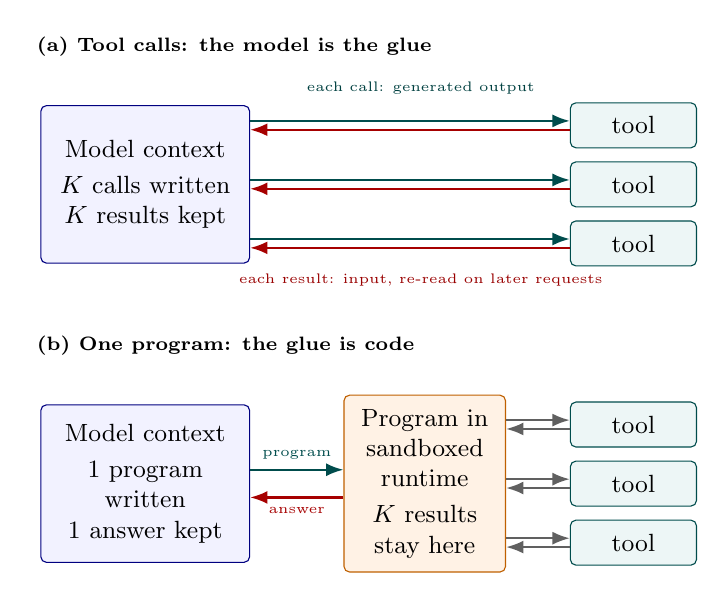
\begin{tikzpicture}[font=\scriptsize]
  % (a) tool calls: every value passes through the model
  \node[font=\scriptsize\bfseries, anchor=west] at (-1.5,1.75) {(a) Tool calls: the model is the glue};
  \node[neutralbox, text width=2.3cm, minimum height=20mm] (m1) at (0,0)
    {Model context\\[2pt]$K$ calls written\\$K$ results kept};
  \foreach \y/\n in {0.75/1, 0/2, -0.75/3} {
    \node[nativebox, text width=1.25cm, minimum height=5mm] (t\n) at (6.2,\y) {tool};
    \draw[flowarrow, teal!60!black] ([yshift=1.6pt]m1.east |- t\n) -- ([yshift=1.6pt]t\n.west);
    \draw[flowarrow, red!65!black] ([yshift=-1.6pt]t\n.west) -- ([yshift=-1.6pt]m1.east |- t\n);
  }
  \node[font=\tiny, teal!50!black, align=center] at (3.5,1.22) {each call: generated output};
  \node[font=\tiny, red!60!black, align=center] at (3.5,-1.22) {each result: input, re-read on later requests};
  % (b) one program: values stay in the runtime
  \node[font=\scriptsize\bfseries, anchor=west] at (-1.5,-2.05) {(b) One program: the glue is code};
  \node[neutralbox, text width=2.3cm, minimum height=20mm] (m2) at (0,-3.8)
    {Model context\\[2pt]1 program written\\1 answer kept};
  \node[codebox, text width=1.7cm, minimum height=20mm] (p) at (3.55,-3.8)
    {Program in\\sandboxed\\runtime\\[2pt]$K$ results\\stay here};
  \foreach \y/\n in {-3.05/4, -3.8/5, -4.55/6} {
    \node[nativebox, text width=1.25cm, minimum height=5mm] (t\n) at (6.2,\y) {tool};
    \draw[flowarrow] ([yshift=1.6pt]p.east |- t\n) -- ([yshift=1.6pt]t\n.west);
    \draw[flowarrow] ([yshift=-1.6pt]t\n.west) -- ([yshift=-1.6pt]p.east |- t\n);
  }
  \draw[flowarrow, teal!60!black] ([yshift=5pt]m2.east) -- node[above, font=\tiny] {program} ([yshift=5pt]p.west);
  \draw[flowarrow, red!65!black] ([yshift=-5pt]p.west) -- node[below, font=\tiny] {answer} ([yshift=-5pt]m2.east);
\end{tikzpicture}%
}
\caption{The idea in one picture.  (a) With tool calls, the model writes each
of the $K$ calls and each result returns to its context: the model carries
every value between tools.  (b) With one program, the calls and their results
stay in the runtime and one value returns.  Clients batch the calls in (a)
into a few model requests, so the two differ little in requests; they differ
in what the model writes and keeps (Table~\ref{tab:tokens}).}
\label{fig:glue}
\end{figure}

The expense is that the model stands in the middle of every hand-off
(Figure~\ref{fig:glue}).  Before
a call can be dispatched, the model must generate it, token by token.  When
the result returns, it joins the conversation and is read again on each later
request.  We call this role \emph{glue}: the model reading and re-emitting
intermediate values only so that they can pass from one tool to the next,
with no decision required of it.  Glue is billed at least twice: as output
when the model writes each call, and as input when each result enters its
context and on every later request that re-reads it.  In the
example, the native arm generates 7.3 times the output tokens of the program
arm and reaches a median peak context of 41.7K tokens against 30.2K, while
the two arms make almost the same number of model requests
(Table~\ref{tab:tokens}).  Context is finite, and what sits in it is paid for
again on each request that re-reads it.  This paper asks when moving glue out
of the model's context pays, and when the model should stay in the loop
because the agent treats each step as a decision of its own.

\paragraph{An idea built in steps.}
Moving glue into a program is not new, and each piece has a source.  CodeAct
showed that a model can act by writing executable code instead of emitting one
structured call at a time, and reported higher task success
\cite{wang2024codeact}.  Cloudflare's Code Mode turned MCP tools into a typed
API that a generated program calls, and ran that program in an isolated
sandbox \cite{cloudflare2025codemode}.  Anthropic showed that tool
definitions need not be loaded until they are needed, and reported a smaller
context \cite{anthropic2025advancedtools,anthropic2025codemcp} and, on its
own evaluations, better tool selection \cite{anthropic2025advancedtools};
Cloudflare then put a
whole API behind two tools, one to search and one to execute
\cite{cloudflare2026codemode}.  The resulting shape --- find a capability,
read only its definition, write a program --- is now a distinct design family
\cite{felendler2026mcp}; it ships in the open-source goose agent
\cite{goose2026codemode} and, for some models, inside a client
(Section~\ref{sec:october}).  Following that literature, we call it
\emph{context-decoupled tool use}: intermediate values are available to the
program without becoming model-visible conversation history.

These reports leave two things open.  First, the common causal story ---
``one program replaces $N$ round trips'' --- predates production clients that
parallelize independent tool calls, cache long prompt prefixes, retrieve tools
on demand, and write large tool results to files.  Those mechanisms change
both sides of the comparison, and static token counts do not reveal billed
cost, generation time, discovery turns, retries, or what the agent actually
chooses to do.  Second, the losses are located only qualitatively.
Felendler et al.\ find plain MCP favored on iterative or adaptive tasks
\cite{felendler2026mcp}.  Anthropic reports roughly 8\% higher cost on a
benchmark whose turns make one or two sequential calls, and advises against
programmatic calling where each call depends on the model reasoning over the
previous result \cite{anthropic2026ptc}.  The goose project's blog states
that for simple single-tool tasks the overhead is not worth it
\cite{goose2026codemode}.  None of these measures where the boundary lies, or
what moves it, under a client that batches and caches.

\paragraph{What the program can reach.}
Those are questions of cost.  A separate question, less examined in priced
comparisons, is reach.  An agent usually reaches MCP tools, which are named
and typed and which most clients permit one at a time, through one mechanism,
and existing command-line programs through another, a shell.  Real tasks
cross that line: the history is in a repository, the record is in a service,
and the rule is in the team's own code.  In a tool-calling agent the model is
again the glue, reading a value from one source and typing it into a request
to the next.  Inside a program the three can share one calling convention.
An MCP tool, a command-line program, and a host function are each a call that
returns a value, although their transports and permission models still
differ.  Some code-mode systems already hand the generated program a shell
tool (Section~\ref{sec:october}).  \toolplane makes a narrower choice.  It
gives an agent a small programmable surface over all three: the agent
searches for a capability, writes a short Python program against awaitable
bindings, and keeps intermediate state in a controlled runtime.  The host,
not the model, owns capability policy, auditing, and the sandbox boundary;
under its allowlist policy a command-line program is exposed one permitted
binary at a time, as a function, not as a shell.
Figure~\ref{fig:example} shows one such program.

We separate these two questions throughout.  Reach is a property of the
interface, and we demonstrate it.  Cost is a measurement, and almost all of
ours use MCP-backed capabilities; the one registered mixed cell, a CLI + MCP
join, did not show a cost advantage (Section~\ref{sec:confirm}).  We
therefore make no cost claim for heterogeneous composition.

\paragraph{The empirical question.}
\emph{Under a modern production agent client, which workload and interface
properties move the observed boundary between native-client tool
orchestration and Toolplane-mediated execution?}  We study that boundary with
\toolplane, an open-source Python code-mode runtime over MCP, CLI, and
host-function capabilities \cite{mcp2025spec,toolplane2026artifact}.
\toolplane is a real interface system and the experimental instrument; the
paper's object is not a universal performance claim about Toolplane, but the
boundary created by this style of programmable mediation.  Every experiment
presents the same underlying MCP fixture to both arms; the treatment is the
agent-facing interface.

Our principal contributions are:

\begin{enumerate}
  \item \textbf{A pre-registered confirmation of the interface boundary.}
  232 runs on Claude Haiku 5.5 at eight per cell, with hypotheses, decision
  rule, and analysis script committed before any data.  Seventeen of 20
  verdicts hold, including \toolplane's losses; two hold only through
  correctness collapses, which we report as such rather than as cost
  results.
  \item \textbf{A mechanism decomposition.}  Request counts and token classes
  show that native clients already batch calls; what \toolplane removes is
  glue: generated call syntax at small payloads and uncached input at large
  ones.
  \item \textbf{Negative and reversed results.}  A native bulk endpoint and
  stepwise chains (including a prose chain built to resist heuristic
  shortcuts) favor the native path; deferred loading leaves only a small
  schema tax; tested hybrid discovery interventions do not generalize; and in
  a second pre-registered study persistent-session reuse turns cost 35\%
  more than conversation reuse, the session's saving coming entirely from the
  load.
  \item \textbf{A reproducible evidence trail.}  Registrations committed
  before data, logged amendments, raw rows, transcripts, frozen-wheel and
  harness hashes, and an explicit record of contaminated or post-hoc-corrected
  measurements, including review changes that should have been logged and
  were not.
\end{enumerate}

These are measurement contributions, not a claim that code execution is a
strictly better tool interface.  Several of the strongest results are losses
for \toolplane.  The guidance they support is conditional but short.  Write a
program when many fine-grained calls, or large intermediate results, would
otherwise pass through the model (the large-payload evidence is four runs
per arm).  Call tools directly for a single lookup, when the agent handles
each step as a separate decision, or when one bulk call already returns
everything.  As a mnemonic, not a decision rule: use the model for judgment,
not for glue.  One caution on the word.  Our chains show agents choosing to
decide step by step, not that those steps required it
(Section~\ref{sec:chain}).  The rest of the paper says how far the evidence
carries that line, and where it stops.

\section{Interfaces and Cost Model}
\label{sec:model}

\subsection{Toolplane as a programmable capability surface}

Figure~\ref{fig:toolplane-surface} summarizes the system shape.  Toolplane
collects heterogeneous capability sources into a searched namespace and exposes
them through a compact MCP facade.  In an agent session, the model can first
discover a relevant capability, then execute Python that calls the selected
binding.  Intermediate variables, loop state, and large payloads can remain in
the runtime namespace; external effects pass through the host adapter that owns
the underlying capability.  This is the design reason Toolplane appears in the
paper: the benchmark is a way to measure the cost and context consequences of
that interface, not the reason the system exists.

\begin{figure}[t]
\centering
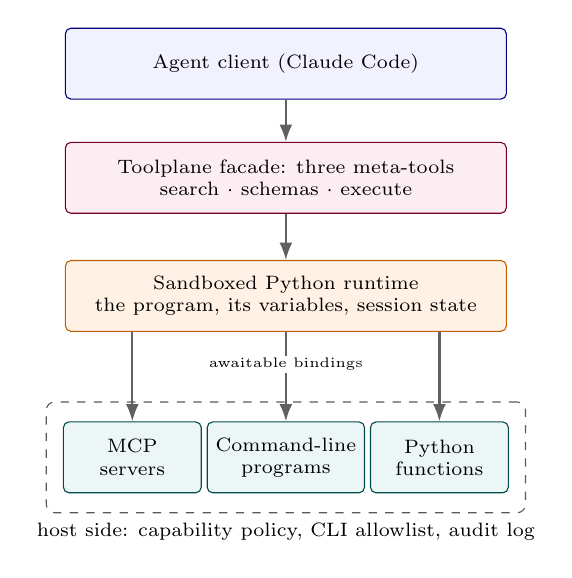
\begin{tikzpicture}[font=\scriptsize,
  box/.style={draw, rounded corners=2pt, align=center, inner sep=4pt,
              minimum height=9mm, minimum width=5.6cm},
  capbox/.style={draw=teal!60!black, fill=teal!7, rounded corners=2pt, align=center,
              inner sep=3pt, minimum height=9mm, minimum width=1.75cm}]
  \node[box, draw=blue!50!black, fill=blue!5] (agent) at (0,0)
    {Agent client (Claude Code)};
  \node[box, draw=purple!60!black, fill=purple!7] (facade) at (0,-1.45)
    {Toolplane facade: three meta-tools\\search $\cdot$ schemas $\cdot$ execute};
  \node[box, draw=orange!75!black, fill=orange!10] (runtime) at (0,-2.95)
    {Sandboxed Python runtime\\the program, its variables, session state};
  \node[capbox] (mcp) at (-1.95,-5.0) {MCP\\servers};
  \node[capbox] (cli) at (0,-5.0) {Command-line\\programs};
  \node[capbox] (py) at (1.95,-5.0) {Python\\functions};
  \node[draw=gray!70!black, dashed, rounded corners=3pt, fit=(mcp)(cli)(py),
        inner xsep=6pt, inner ysep=7pt] (host) {};
  \node[font=\scriptsize, anchor=north] at (host.south)
    {host side: capability policy, CLI allowlist, audit log};
  \draw[flowarrow] (agent) -- (facade);
  \draw[flowarrow] (facade) -- (runtime);
  \draw[flowarrow] (runtime.south -| mcp) -- (mcp.north);
  \draw[flowarrow] (runtime.south -| cli) -- (cli.north);
  \draw[flowarrow] (runtime.south -| py) -- (py.north);
  \node[font=\tiny, fill=white, inner sep=1pt] at (0,-3.82) {awaitable bindings};
\end{tikzpicture}
\caption{Toolplane as a compact programmable surface.  The agent sees three
meta-tools; a program it writes runs in the sandbox and reaches capabilities
only through bindings the host exposes.  The benchmark isolates MCP-backed
capabilities, but the same surface mediates command-line programs and
host/Python functions.}
\label{fig:toolplane-surface}
\end{figure}

\subsection{Two interfaces over the same capabilities}

In the \emph{native} arm, an MCP server's operations are registered natively as
ordinary model-callable tools.  In the \toolplane arm, the same server is
registered behind three Toolplane meta-tools: capability search, schema
inspection, and Python execution.  The labels are shorthand for two
end-to-end treatments, not pure paradigms.  In particular, the native-client
arm may use Claude Code built-ins, batch calls, or externalize a large result
to a file and process it with code; the Toolplane arm may also use client
built-ins unless a task-specific matrix disables them.  The executor exposes
async bindings such as
\texttt{await orders\_get\_order(order\_id=...)}.  The default Monty runtime
has no filesystem or network access; external effects pass through audited
host bindings.  Session variables may persist across executions, and a
pre-execution snapshot allows namespace rollback after timeout.
Figure~\ref{fig:glue} shows the two paths side by side.


\paragraph{An illustration of reach.}
Figure~\ref{fig:example} makes the surface concrete.  The question is which
enterprise customers have waited too long for a fix that a release finally
ships.  The commits are in a repository, the tickets and the customers are in
two services, and the escalation rule is a Python function.  One program
reads the history, fetches each ticket, asks the second service only when the
branch requires it, and applies the rule.  In a recorded run it made 181
capability calls and returned one value of 419 bytes, computed from 24,990
bytes of tool results that stayed inside the runtime.  We wrote this
program and ran it through \toolplane's library interface; no agent was
involved and it is not a benchmark cell.  It illustrates what the surface can
express.  Whether agents write such programs unprompted is a separate
question, on which our evidence is mixed (Sections~\ref{sec:confirm}
and~\ref{sec:october}).

\begin{figure}[t]
\begin{lstlisting}[language=Python,basicstyle=\ttfamily\scriptsize,breaklines=true,columns=fullflexible,frame=single,showstringspaces=false]
import re
log = await git("log", format="%s", _=["v1.4..HEAD"])
ids = re.findall(r"TCK-\d+", log["stdout"])
pending = [tickets_get_ticket(id=i) for i in ids]
hits = []
for p in pending:
    ticket = await p
    if ticket["reported_by_customer"]:
        customer = await customers_get_customer(
            id=ticket["customer_id"])
        if await policy_sla_breach(ticket=ticket,
                                   customer=customer):
            hits.append({"customer": customer["name"],
                         "ticket": ticket["id"]})
return {"commits": len(ids), "fixed_for": hits}
\end{lstlisting}
\caption{Author-written interface illustration; no agent and no cost
comparison.  One program over three kinds of capability: a command-line program
(\texttt{git}), two MCP servers (\texttt{tickets}, \texttt{customers}), and a
host Python function (\texttt{policy\_sla\_breach}).  Recorded run against
fixture data: 1 CLI call, 140 MCP calls, 40 function calls; the conditional
skips 60 of 100 possible calls to the second server.  An illustration of
reach; line breaks added for the column.  No cost is claimed for it.  The
program, fixtures and the script that records the run are in
\texttt{pitch/example/} in the repository.}
\label{fig:example}
\end{figure}

\subsection{A qualitative boundary, not a fitted law}

Let $K$ be the number of external capability invocations required by the API
shape, $P$ the payload returned per invocation, $A$ the number of sequential
judgment stages, $M$ the registered-server surface, and $T$ the number of
related user turns.  For treatment $j$, a useful decomposition is

\begin{align}
C_j \approx {}& F_j(M) + c_o O_j(K,A)
 + c_u I_{u,j}(K,P,T) \\
&+ c_w I_{w,j}(K,P,T) + c_r I_{r,j}(K,P,T)
 + C_{\mathrm{retry},j},
\end{align}

where $F$ is fixed discovery/interface cost, $O$ is model-generated output,
$I_u$, $I_w$, and $I_r$ are uncached input, cache-write input, and cache-read
input, and $c_o,c_u,c_w,c_r$ are their provider prices.  Client behavior gates
which result bytes enter any input class: a result may be inlined, cached,
trimmed, or externalized to a file.  This is explanatory notation, not a
regression model; those gates and agent choices are discontinuous and
client-specific.  Wall time adds another term.  If native calls batch while
sandbox external awaits serialize, the Toolplane arm approaches a $K\ell$
sequential critical path, whereas the native arm pays the client's batched
critical path plus its own generation and dispatch overhead.  On an
eager-dispatch runtime the sandbox term is idiom-dependent: firing calls
before awaiting them collapses the $K\ell$ path to roughly $\ell$ plus
dispatch, so the wall comparison also depends on whether the agent writes
that idiom.

These terms make glue classifiable.  Two token classes are glue: output
spent generating calls whose arguments are fixed by the task or copied from
earlier results (the part of $O_j$ that scales with $K$), and input carrying
intermediate results that the answer does not need verbatim (the part of the
input classes that scales with $K$ and $P$).  Two are not.  $F_j$, the fixed
cost of either route, is paid whether or not there is anything to carry, and
it is why a single lookup favors the native path.  And $A$ counts the stages
the agent handles as separate decisions.  Moving glue into a program removes
most of the first two; it cannot remove $F_j$, and the decision stages remain
wherever the agent decides step by step.  The fetch-one scale and payload
cells measure the two glue classes, the single lookup measures $F_j$, the
chains measure $A$, and the bulk cells remove $K$ on both sides.

The experiments vary one or two of these axes at a time.  The object of study
is the sign and mechanism of
$\Delta=C_{\mathrm{native}}-C_{\mathrm{Toolplane}}$, not a universal coefficient.

The rest of the paper follows four questions: how interaction scale changes the
winner; how payload, API granularity, task structure, and latency move the
boundary; how client mediation and discovery affect cost; and whether
persistent Toolplane sessions create savings beyond ordinary conversation
reuse, and where those savings come from.

\section{Methodology}
\label{sec:methods}

Every experiment gives both arms the same task, fixture, and prompt; only the
agent-facing interface differs.  This section says how runs were produced and
how much weight each carries.

\subsection{System under test}

The study ran in epochs (Table~\ref{tab:epochs}).  A July pilot on Claude
Sonnet 5 found the boundary's shape through successive interventions.  In
October, two pre-registered studies re-tested its main claims on the shipped
runtime, and smaller replications probed a second client and new fixtures.
\textbf{Epoch rule:} pre-registered October cells are the primary evidence;
July cells are the pilot; no table or ratio combines models or epochs, and
every table caption names its model.  Client version is part of the
treatment, so wall times are not compared across versions.  Per-row wheel
hashes pin the served bytes.  The benchmark runs in fresh scratch directories
with strict MCP configuration.  Later task-specific matrices disable Bash,
file, web, and helper-agent shortcuts where isolation is required; other
matrices retain client-selected built-ins and disclose their use.

\begin{table*}[t]
\centering
\scriptsize
\caption{Experimental epochs.  ``Registered'' means hypotheses, decision rule
and analysis script were committed before any data.}
\label{tab:epochs}
\begin{tabular}{>{\raggedright\arraybackslash}p{0.17\linewidth}>{\raggedright\arraybackslash}p{0.17\linewidth}>{\raggedright\arraybackslash}p{0.15\linewidth}>{\raggedright\arraybackslash}p{0.13\linewidth}>{\raggedright\arraybackslash}p{0.10\linewidth}>{\raggedright\arraybackslash}p{0.14\linewidth}}
\toprule
Epoch & Model & Client & Runtime & Design & Backs \\
\midrule
July pilot & Claude Sonnet 5 & Claude Code 2.1.204--2.1.207 & pre-release; Monty 0.0.18 (latency cells 0.0.19 beta) & 2--4 runs, adaptive & mechanisms, hybrid, naming, session pilot \\
October replications & Sonnet 5; Sonnet 5.5; Haiku 5.5; Codex gpt-5.5 and gpt-6.1-sol & Claude Code 2.1.293--2.1.295; Codex CLI 0.160.0 & \toolplane 0.5.x; Monty 1.1 & 4 runs (abstention follow-up 60 and 40) & runtime re-run, second client, prose chain, CLI join \\
Confirmation matrix & Claude Haiku 5.5 (Sonnet 5.5 slice, 2 runs) & Claude Code 2.1.296 & 0.5.2 wheel; Monty 1.1 & registered, 8 runs & primary cost envelope (Section~\ref{sec:confirm}) \\
Persistence study & Claude Sonnet 5.5 & Claude Code 2.1.296 & same wheel & registered, 8 sessions; 8-run slice & primary session results (Section~\ref{sec:sessions}); single and chain on Sonnet 5.5 \\
\bottomrule
\end{tabular}
\end{table*}

The deterministic fixture is an order store with formula-generated records.
Its minimal interface lists record identifiers and fetches one record.  Later
experiments add mutually exclusive bulk retrieval, synthetic answer-irrelevant
detail padding of 2,000 or 20,000 characters per record, latency, templated
note chains, and semantically distant distractor servers.  Both arms
receive byte-identical task prompts and data.  Correct answers are computed
from the shared fixture and validated programmatically.  Although Toolplane can
also mediate CLI commands and Python or host functions, the paid experiments
exercise its MCP branch so the native and Toolplane arms share the same
underlying external operations.

\begin{table*}[t]
\centering
\small
\caption{Controlled experimental axes.  ``Production behavior'' means the
client mechanism is observed rather than disabled or simulated.}
\label{tab:axes}
\begin{tabular}{>{\raggedright\arraybackslash}p{0.22\linewidth}>{\raggedright\arraybackslash}p{0.31\linewidth}>{\raggedright\arraybackslash}p{0.37\linewidth}}
\toprule
Axis & Levels & Purpose \\
\midrule
Interactions $K$ & single lookup; loops of 5, 10, 20, 30, 100 & Observe the
small-task loss and transition across experimental epochs \\
Task structure & independent loop; four-hop templated chain & Compare bulk
composition with the stepwise strategy agents selected \\
Payload $P$ & baseline, 2~KB, 20~KB synthetic detail per record & Measure
context isolation under controlled payload growth \\
API granularity & fetch-one; bulk & Give the native-client arm a realistic batching
affordance \\
Latency $\ell$ & 0; 100~ms per call & Expose batched native calls against the
sandbox critical path (serial awaits, then taught fan-out) \\
Registry $M$ & 1, 5, 15 servers & Test schema/catalog scaling under deferred
loading \\
Interface & native; Toolplane; hybrid; curated hybrid & Test routing and discovery
interventions \\
Session turns $T$ & initial load; four reuse turns; reset/refetch & Test
persistent state, refetching, and context growth \\
Snapshot state & 1~KB, 100~KB, 10~MB & Bound rollback checkpoint overhead \\
\bottomrule
\end{tabular}
\end{table*}

\subsection{Metrics}

For every paid run we record task correctness, billed US-dollar cost, wall
time, output tokens, uncached input (input plus cache creation), cache reads,
and tool-use blocks.  Complete transcripts are kept from the hardened harness
onward; the first interaction-scale and registry-size matrices predate it.  Hardened
harness versions additionally count unique model request identifiers, peak
request-context tokens, discovery events, execution errors versus staged
calls, fixture-server calls, and client startup artifacts.  Cost is the
client-reported billed total and therefore includes asymmetric cache reads.
Cost-of-pass is total spend divided by successful runs; all headline matrices
reported here have full correctness unless noted.

The registered studies report a 95\% percentile bootstrap interval (4,000
resamples, seed 0, each arm resampled independently) on the difference in
cost of pass, with a timed-out run priced at its cell's highest observed cost.
A directional prediction holds when the interval excludes zero in the
predicted direction and is reversed when it excludes zero in the other.
Pilot cells have two to four repetitions and are reported as medians and
observed ranges; there, range overlap is descriptive, not evidence of
equivalence, and arm differences are called unresolved where ranges
overlap.  The discovery naming A/B uses
larger pooled samples but remains exploratory because agent-generated search
queries vary by arm.

We distinguish evidence tiers in the synthesis.  The two registered October
studies are primary evidence.  The July payload-by-granularity matrix and
longitudinal pilot (frozen code, three or four repetitions) and the October
four-repetition replications are secondary.  So are the July crossover,
templated chain, latency, registry, and hybrid studies, which used smaller
samples or earlier harness epochs.  The naming/description A/B and
pre-hardening pilots are exploratory.  Later rigor does not retroactively
upgrade earlier runs.

These tiers are a claim-management device rather than a statistical
correction.  Primary evidence anchors the paper's cost and context
conclusions; secondary studies support mechanism probes and the envelope; and
exploratory rows are used only for hypotheses and provenance.  Appendix
\ref{app:evidence-tiers} records the full tier map.

\subsection{Provenance and experimental epochs}

The July pilot accumulated through successive interventions rather than one
frozen matrix; the October studies were registered instead.  For those, the
commit that adds the plan (\texttt{bench/PREREG-*.md}) is the registration,
and later changes are logged as amendments.  The confirmation matrix has one
amendment (A1, before the main run): it dropped one block whose projected cost
exceeded the target and the longitudinal block after Claude Haiku 5.5
degenerated on its calibration fixture, cut the 20~KB cells to four runs, and
cut the Sonnet 5.5 slice to two runs per arm.  Four review commits that tightened its rules
before any data were not logged as amendments at the time; its results
document discloses them, and an independent recompute found that none changes
a verdict.  Early results exposed harness and product defects; later
runs serve from a built wheel, stamp source and fixture hashes, alternate or
balance arm order, persist transcripts, and count request IDs directly.  Paid
matrices are never edited while running.  Result rows record Git SHA and dirty
state.

Four exceptions are retained and disclosed in Appendix~\ref{app:reset}: a
contaminated matrix, a rescored validator, naming runs from an uncommitted
tree, and corrected per-turn token fields.  None changes a primary table.

The artifact contains full prompts, harness code, raw JSON, validators,
classification scripts, and the registrations and results documents of both
October studies; Appendices~\ref{app:evidence-tiers} and~\ref{app:artifacts}
map each result to its artifact.  For
matrices run on the hardened harness it also contains complete
transcript-level tool inputs and outputs and exact request IDs; the two
earliest pilots predate that.  Secrets and irrelevant client-environment fields are redacted;
behavioral evidence is retained.

\subsection{Scope of inference}

Our treatment is an end-to-end client/model/interface system.  Claude Code's
retrieval, batching, caching, built-ins, and result-file behavior are part of
the measured system, not nuisance variables that can be subtracted after the
fact.  Consequently, the clean frozen two-arm interventions support
within-system mechanism claims, while early fixed-order and outcome-adaptive
experiments are treated as exploratory.  The registered cost envelope is on
Claude Haiku 5.5; the registered session results and an eight-run Sonnet 5.5
slice (chain loss holds, single lookup unresolved) are on Claude Sonnet 5.5.
Four-run Codex replications point the same way but are not registered
evidence.  Generalization beyond these
client--model pairs is not established.  Synthetic tasks make mechanisms
inspectable but do not estimate a population of real user workloads.


\section{Primary Results}
\label{sec:primary-results}

Two pre-registered October studies carry the main claims: a 240-run
confirmation matrix (232 runs on Claude Haiku 5.5) for the cost envelope, and a 24-session
longitudinal study on Claude Sonnet 5.5 for persistence.  The July payload
matrix follows as the pilot that motivated the matrix's payload hypotheses.

\subsection{Pre-registered confirmation matrix (Claude Haiku 5.5)}
\label{sec:confirm}

The matrix (232 Claude Haiku 5.5 runs, plus a two-run Claude Sonnet 5.5 slice
reported as descriptive only) re-tests the pilot's claims on the shipped runtime (the
\toolplane 0.5.2 wheel, Monty 1.1) with Claude Code 2.1.296.  Claude Haiku 5.5
was chosen because it costs about a seventeenth as much per run as Claude
Sonnet 5.5 on the same task, which pays for eight runs per arm per cell.  The
20~KB cells have four.  Arm order alternates by repetition.  The registration
(\texttt{bench/PREREG-confirmation-2026-10.md}) fixed each hypothesis, the
cells it reads, the decision rule (Section~\ref{sec:methods}), and the
analysis script before any data.  All 240 rows are clean and uniform in code
and wheel, and every row that reported a client version reports 2.1.296 (three
timeouts report none).  The rows record \usd{4.81}, excluding the three
timeouts, whose cost the client never reported.

\begin{table*}[t]
\centering
\scriptsize
\caption{Registered verdicts, Claude Haiku 5.5, eight runs per arm unless
noted.  Ratio is \toolplane{} cost of pass over native; the interval is the
95\% bootstrap CI of the difference in USD per correct answer.}
\label{tab:confirm}
\resizebox{\textwidth}{!}{%
\begin{tabular}{llrll}
\toprule
ID & Cell & Ratio & Difference, 95\% CI & Verdict \\
\midrule
H1a & single lookup & 1.11 & +.0005 [+.0003, +.0008] & holds: native cheaper \\
H1b & loop, $N=5$ & 1.13 & +.0006 [+.0002, +.0011] & holds: native cheaper \\
--- & loop, $N=20$ (not tested) & 0.93 & --- & --- \\
H3 & loop, $N=30$, fetch-one, no padding & 0.82 & $-$.0012 [$-$.0015, $-$.0009] & holds: \toolplane cheaper \\
H2a & loop, $N=100$ & 0.50 & $-$.0059 [$-$.0065, $-$.0053] & holds: \toolplane cheaper \\
H3 & fetch-one, 2~KB/record & --- & native 0/8 correct & holds, \textbf{by a correctness collapse} \\
H3 & fetch-one, 20~KB/record (4 runs) & 0.020 & $-$.392 [$-$.403, $-$.382] & holds: \toolplane cheaper \\
H4 & bulk, 0 / 2~KB / 20~KB (4 runs) & 1.24 / 1.05 / 1.31 & all intervals $\geq 0$ & holds $\times$3: native cheaper \\
H5 & templated / prose chain & 1.12 / 1.12 & +.0007 [+.0006, +.0009]; +.0008 [+.0005, +.0011] & holds $\times$2: native cheaper \\
H6a & 100~ms latency, wall time & --- & $-$1.45~s [$-$3.60, +1.35] & \textbf{unresolved} \\
H6b & 100~ms latency, cost & 0.91 & $-$.0006 [$-$.0009, $-$.0003] & holds: not costlier \\
H7a & CLI + MCP join, no shell & 1.12 & +.0008 [$-$.00003, +.0016] & \textbf{unresolved}, point against \\
H7b & CLI + MCP join, shell available & 4.47 & \toolplane 2/8 correct & holds, \textbf{by a correctness collapse} \\
H8 & native at $M=15$ vs $M=1$ & 1.03 & +.0002 [+.00003, +.0003] & \textbf{reversed}, inside the $\pm$10\% margin \\
\bottomrule
\end{tabular}%
}
\end{table*}

Table~\ref{tab:confirm} condenses the 20 tested Haiku rows (omitting the two
slope hypotheses, the payload-growth contrast, and the hop-by-hop walk check,
all of which hold): 17 hold, two are unresolved, and one is reversed.  The
two-run Sonnet 5.5 slice is not counted; with two runs per arm its interval
is not a real one.  The shape is the pilot's
(Figure~\ref{fig:curve}).  \toolplane loses
a single lookup and a five-record loop by 11--13\%, wins from somewhere
between 5 and 20 records (20 itself was run but not tested), and costs half as
much at 100.  Toolplane's per-record slope is about 15 times flatter than
native's, but not zero.  A native bulk endpoint and both stepwise chains
reverse the winner.  Four verdicts cannot be cited bare.

\begin{figure}[t]
\centering
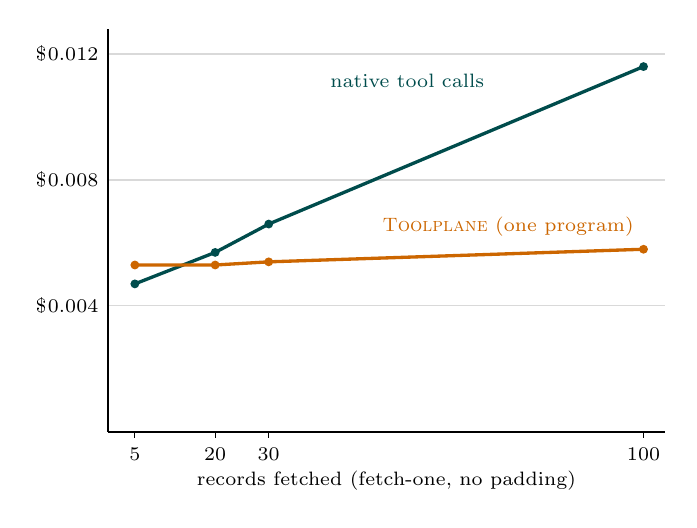
\begin{tikzpicture}
  \draw[gray!30] (0,1.6) -- (7.072,1.6);
  \node[left, font=\scriptsize] at (0,1.6) {\$0.004};
  \draw[gray!30] (0,3.2) -- (7.072,3.2);
  \node[left, font=\scriptsize] at (0,3.2) {\$0.008};
  \draw[gray!30] (0,4.8) -- (7.072,4.8);
  \node[left, font=\scriptsize] at (0,4.8) {\$0.012};
  \draw[thick] (0,0) -- (7.072,0);
  \draw[thick] (0,0) -- (0,5.12);
  \draw (0.34,0) -- (0.34,-0.08) node[below, font=\scriptsize] {5};
  \draw (1.36,0) -- (1.36,-0.08) node[below, font=\scriptsize] {20};
  \draw (2.04,0) -- (2.04,-0.08) node[below, font=\scriptsize] {30};
  \draw (6.8,0) -- (6.8,-0.08) node[below, font=\scriptsize] {100};
  \node[font=\scriptsize] at (3.536,-0.62) {records fetched (fetch-one, no padding)};
  \draw[very thick, teal!60!black] (0.34,1.88) -- (1.36,2.28) -- (2.04,2.64) -- (6.8,4.64);
  \draw[very thick, orange!80!black] (0.34,2.12) -- (1.36,2.12) -- (2.04,2.16) -- (6.8,2.32);
  \fill[teal!60!black] (0.34,1.88) circle (1.6pt);
  \fill[orange!80!black] (0.34,2.12) circle (1.6pt);
  \fill[teal!60!black] (1.36,2.28) circle (1.6pt);
  \fill[orange!80!black] (1.36,2.12) circle (1.6pt);
  \fill[teal!60!black] (2.04,2.64) circle (1.6pt);
  \fill[orange!80!black] (2.04,2.16) circle (1.6pt);
  \fill[teal!60!black] (6.8,4.64) circle (1.6pt);
  \fill[orange!80!black] (6.8,2.32) circle (1.6pt);
  \node[above left, font=\scriptsize, teal!60!black] at (4.9,4.25) {native tool calls};
  \node[above left, font=\scriptsize, orange!80!black] at (6.8,2.36) {\toolplane{} (one program)};
\end{tikzpicture}
\caption{Cost per correct answer against records fetched, Claude Haiku 5.5,
eight runs per arm (cell values from the registered analysis output; the
20-record cell was run but not tested).  Native cost rises with each
generated call; \toolplane{} pays a fixed interface cost and a slope about 15
times flatter.  The single lookup is a different task and is not plotted.}
\label{fig:curve}
\end{figure}

\paragraph{H3 at 2~KB is a collapse, not a cost.}  All eight native runs
fetched the 30 records and then degenerated while combining them: three timed
out at 900~s, three ended without an answer, one answered in gibberish, and one
ended in a usage-policy refusal.  The five that finished produced 60K--259K
output tokens.  The 20~KB native runs saw the same repeated-token padding,
ten times larger, and passed 4/4, so ``more payload, more failure'' does not
explain it; the cause is not isolated.  The verdict holds under the
registered rule because failures are priced into cost of pass, but it says
nothing about token economics at 2~KB.

\paragraph{H7b holds through a skipped search.}  With a shell available,
every run in both arms first read the repository through Bash.  All eight
native runs then called the client's \texttt{ToolSearch}, found the order
tool, and passed.  Six of eight \toolplane runs never searched, concluded the
amounts were unreachable, and answered without them.  A failed \toolplane run
cost about what a native run did, so the 4.47 ratio is a correctness result.
Without a shell (H7a), \toolplane passed 8/8 at 1.12$\times$ native; the
interval just crosses zero.  On Sonnet 5.5 the same configuration measured
0.94$\times$ in October (Section~\ref{sec:october}), so the CLI join's cost
advantage does not replicate on Haiku.

\paragraph{H8: a small schema tax.}  The registration predicted no cost
difference for native tools between 1 and 15 configured servers, within
$\pm$10\%.  The measured difference is +3\%, with an interval wholly inside
the margin but excluding zero.  The registered code checked ``excludes zero''
before the margin, so the verdict is reversed.  The plain reading is a
detectable but small schema tax at $M=15$.  Later registrations test the
margin first.

\paragraph{H6a: concurrency is unresolved on wall time.}  With 100~ms of
latency per call and the fan-out idiom taught in the executor's description,
\toolplane's median wall time is 1.45~s lower, but the interval spans zero.
The pilot's wall-time win (Section~\ref{sec:latency}) is not confirmed.  The
cost side holds: \toolplane was not costlier.

\paragraph{The registered Sonnet 5.5 slice.}  The persistence study
(Section~\ref{sec:sessions}) re-ran two cells on Claude Sonnet 5.5 at eight
runs per arm.  The chain loss holds: \toolplane costs 1.03$\times$ native on
the prose chain ($+$\usd{0.0030} [$+$0.0013, $+$0.0049]).  The single-lookup
loss is unresolved ($-$\usd{0.0026} [$-$0.0133, $+$0.0030]).  Costs there are
nearly deterministic --- seven native runs cost exactly \usd{0.0711} and seven
\toolplane runs \usd{0.0732} --- but the first run of the block paid prompt-cache
creation (\usd{0.1123}) and alone moves the native mean below \toolplane's.
The registration allows no exclusions, so the verdict stays unresolved.

\begin{table}[t]
\centering
\scriptsize
\caption{Where the cost goes: median token classes per run, Claude Haiku 5.5,
native / \toolplane.  Uncached input includes cache writes; peak is the
largest single-request context.}
\label{tab:tokens}
\resizebox{\linewidth}{!}{%
\begin{tabular}{lrrrrr}
\toprule
Cell & Output & Uncached input & Cache read & Peak context & Requests \\
\midrule
single & 203 / 318 & 16.6K / 18.0K & 64.4K / 66.0K & 27.2K / 28.6K & 3 / 3 \\
$N=30$ & 2,946 / 1,082 & 20.7K / 20.0K & 92.1K / 96.5K & 31.2K / 30.6K & 4 / 4 \\
$N=100$ & 8,178 / 1,127 & 31.1K / 19.7K & 132.8K / 97.7K & 41.7K / 30.2K & 5 / 4 \\
20~KB, $N=30$ & 3,456 / 1,496 & 396.4K / 27.1K & 295.2K / 127.7K & 407.0K / 37.6K & 4.5 / 5 \\
\bottomrule
\end{tabular}%
}
\end{table}

\begin{figure}[t]
\centering
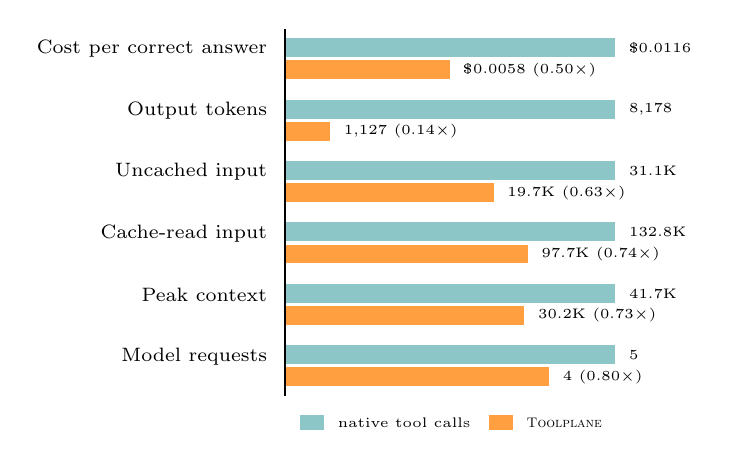
\begin{tikzpicture}
  \node[anchor=east, font=\scriptsize] at (-0.1,-0.14) {Cost per correct answer};
  \fill[teal!45] (0,0.00) rectangle (4.2,-0.24); \node[anchor=west, font=\tiny] at (4.25,-0.12) {\$0.0116};
  \fill[orange!75] (0,-0.28) rectangle (2.100,-0.52); \node[anchor=west, font=\tiny] at (2.150,-0.40) {\$0.0058 (0.50$\times$)};
  \node[anchor=east, font=\scriptsize] at (-0.1,-0.92) {Output tokens};
  \fill[teal!45] (0,-0.78) rectangle (4.2,-1.02); \node[anchor=west, font=\tiny] at (4.25,-0.90) {8,178};
  \fill[orange!75] (0,-1.06) rectangle (0.579,-1.30); \node[anchor=west, font=\tiny] at (0.629,-1.18) {1,127 (0.14$\times$)};
  \node[anchor=east, font=\scriptsize] at (-0.1,-1.70) {Uncached input};
  \fill[teal!45] (0,-1.56) rectangle (4.2,-1.80); \node[anchor=west, font=\tiny] at (4.25,-1.68) {31.1K};
  \fill[orange!75] (0,-1.84) rectangle (2.654,-2.08); \node[anchor=west, font=\tiny] at (2.704,-1.96) {19.7K (0.63$\times$)};
  \node[anchor=east, font=\scriptsize] at (-0.1,-2.48) {Cache-read input};
  \fill[teal!45] (0,-2.34) rectangle (4.2,-2.58); \node[anchor=west, font=\tiny] at (4.25,-2.46) {132.8K};
  \fill[orange!75] (0,-2.62) rectangle (3.089,-2.86); \node[anchor=west, font=\tiny] at (3.139,-2.74) {97.7K (0.74$\times$)};
  \node[anchor=east, font=\scriptsize] at (-0.1,-3.26) {Peak context};
  \fill[teal!45] (0,-3.12) rectangle (4.2,-3.36); \node[anchor=west, font=\tiny] at (4.25,-3.24) {41.7K};
  \fill[orange!75] (0,-3.40) rectangle (3.045,-3.64); \node[anchor=west, font=\tiny] at (3.095,-3.52) {30.2K (0.73$\times$)};
  \node[anchor=east, font=\scriptsize] at (-0.1,-4.04) {Model requests};
  \fill[teal!45] (0,-3.90) rectangle (4.2,-4.14); \node[anchor=west, font=\tiny] at (4.25,-4.02) {5};
  \fill[orange!75] (0,-4.18) rectangle (3.360,-4.42); \node[anchor=west, font=\tiny] at (3.410,-4.30) {4 (0.80$\times$)};
  \draw[thick] (0,0.12) -- (0,-4.54);
  \fill[teal!45] (0.2,-4.78) rectangle (0.5,-4.98); \node[anchor=west, font=\tiny] at (0.55,-4.88) {native tool calls};
  \fill[orange!75] (2.6,-4.78) rectangle (2.9,-4.98); \node[anchor=west, font=\tiny] at (2.95,-4.88) {\toolplane};
\end{tikzpicture}
\caption{Where the saving is, at 100 records (Claude Haiku 5.5, medians of
eight runs per arm; each pair is scaled to native $=1$).  Requests barely
differ.  The model's own output falls to about a seventh, and the input
classes fall by a quarter to a third.}
\label{fig:classes}
\end{figure}

\paragraph{What the model pays for.}  Table~\ref{tab:tokens} applies
the cost model's terms to the registered rows.  Request counts barely differ:
the client batches native calls, so \toolplane does not win by saving round
trips.  Without padding, the native arm's extra cost is output: one generated
call block per record, 2.7 times \toolplane's output at $N=30$ and 7.3 times
at $N=100$ (Figure~\ref{fig:classes}).  At 20~KB per record the extra cost moves to input: every record
enters native context, and uncached input is 14.6 times \toolplane's.  On a
single lookup \toolplane is slightly larger on every token class, which is the
fixed interface cost.  This is the glue of the introduction, measured: calls
the model had to write, and results it had to hold, so that values could move
between tools.

\finding{On Claude Haiku 5.5, \toolplane costs 11--13\% more on small tasks, half as
much at 100 fine-grained calls, and a fiftieth when those calls return 20~KB
records; a bulk endpoint or a stepwise chain reverses the winner.  The saving
is what the model no longer writes and holds, not fewer requests.}

\subsection{Persistent sessions are front-loaded; reuse turns cost more}
\label{sec:sessions}

All earlier tasks start fresh.  Sessions ask whether the saving survives
reuse: once records are in the sandbox, does each later question still pay
for them?  The longitudinal experiment keeps one Claude
Code process and one MCP process alive across six user turns over 30 records
padded by 2~KB: initial load and totals, four related filters/aggregates
(reuse turns), and a separately scored reset/refetch contract.  Bash, files,
web, and helper agents are disabled.  Turn 6 forces \toolplane to reset and
refetch while the native client has no analogous operation, so the economic
comparison uses turns 1--5 only.

Two studies use this fixture.  A July pilot on Claude Sonnet 5 (four
counterbalanced runs per arm, two arms, repeated-token record padding) is
exploratory.  A pre-registered study on Claude Sonnet 5.5
(\texttt{PREREG-persistence-2026-10.md}; hypotheses, decision rule and
analysis script committed before any data) is the primary evidence.  It runs
eight counterbalanced sessions per arm with varied-word padding and three arms:
native client; \toolplane with its default persistent Monty session; and
\toolplane with sessions off but the result store
(\texttt{save\_result}/\texttt{load\_result}) on --- the shipped alternative,
not a no-memory arm.  Verdicts use a 95\% percentile bootstrap (4,000
resamples) on differences of per-arm medians.  Equivalence is tested margin
first: a CI wholly inside $\pm$10\% of the reference median holds.  All 24
sessions passed turns 1--5, none died, and every row is clean and uniform in
code, client version, and model.

\begin{table*}[t]
\centering
\scriptsize
\caption{Pre-registered longitudinal results on Claude Sonnet 5.5, turns 1--5,
eight sessions per arm, median [observed range].  Costs in USD.  The last
column gives the registered verdict for the \toolplane~$-$~native difference
with its 95\% bootstrap CI.  ``Sessions off'' is \toolplane with the Monty
session disabled and the result store on.}
\label{tab:session}
\begin{tabular}{lrrrl}
\toprule
Metric & Native & \toolplane & Sessions off & \toolplane $-$ native, 95\% CI \\
\midrule
Cumulative cost & .195 [.194, .195] & \textbf{.116 [.112, .125]} & .125 [.123, .127] & $-$.078 [$-$.082, $-$.073], holds ($-$40\%) \\
Peak request context & 44.2K [44.2, 44.2] & \textbf{27.5K [26.6, 28.2]} & 28.4K [28.0, 28.5] & $-$16.7K [$-$17.5, $-$16.3], holds ($-$38\%) \\
Initial load + totals & .170 [.170, .170] & \textbf{.085 [.079, .087]} & .086 [.086, .088] & not tested ($-$50\%) \\
Reuse turns 2--5 & \textbf{.0245 [.0240, .0250]} & .0330 [.0317, .0382] & .0381 [.0372, .0393] & +.0086 [+.0077, +.0102], \textbf{reversed} (+35\%) \\
Requests per reuse turn & 1 & 2 & 2 & --- \\
\bottomrule
\end{tabular}
\end{table*}

\begin{figure}[t]
\centering
\resizebox{\linewidth}{!}{%
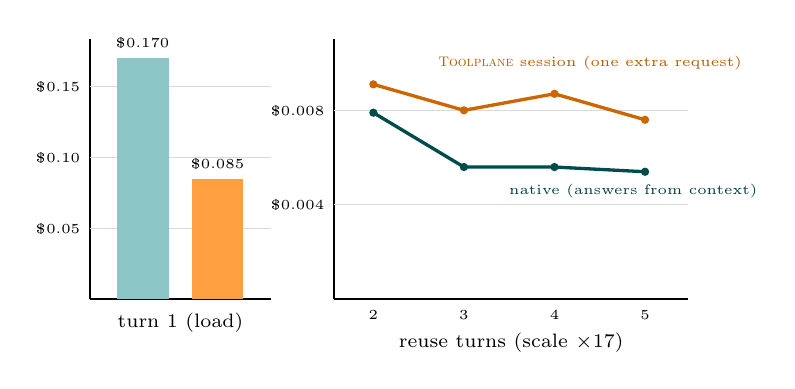
\begin{tikzpicture}
  % load turn
  \draw[thick] (0,0) -- (2.3,0); \draw[thick] (0,0) -- (0,3.3);
  \foreach \v in {0.05,0.10,0.15} { \draw[gray!30] (0,\v*18) -- (2.3,\v*18); \node[left, font=\tiny] at (0,\v*18) {\$\v}; }
  \fill[teal!45] (0.35,0) rectangle (1.0,3.067); \node[above, font=\tiny] at (0.675,3.067) {\$0.170};
  \fill[orange!75] (1.3,0) rectangle (1.95,1.523); \node[above, font=\tiny] at (1.625,1.523) {\$0.085};
  \node[below, font=\scriptsize] at (1.15,-0.05) {turn 1 (load)};
  % reuse turns, own scale
  \draw[thick] (3.1,0) -- (7.6,0); \draw[thick] (3.1,0) -- (3.1,3.3);
  \foreach \v in {0.004,0.008} { \draw[gray!30] (3.1,\v*300) -- (7.6,\v*300); \node[left, font=\tiny] at (3.1,\v*300) {\$\v}; }
  \foreach \t in {2,3,4,5} { \node[below, font=\tiny] at ({3.6+(\t-2)*1.15},-0.02) {\t}; }
  \node[below, font=\scriptsize] at (5.35,-0.3) {reuse turns (scale $\times$17)};
  \draw[very thick, teal!60!black] (3.600,2.370) -- (4.750,1.680) -- (5.900,1.680) -- (7.050,1.620);
  \draw[very thick, orange!80!black] (3.600,2.730) -- (4.750,2.400) -- (5.900,2.610) -- (7.050,2.280);
  \fill[teal!60!black] (3.600,2.370) circle (1.5pt); \fill[orange!80!black] (3.600,2.730) circle (1.5pt);
  \fill[teal!60!black] (4.750,1.680) circle (1.5pt); \fill[orange!80!black] (4.750,2.400) circle (1.5pt);
  \fill[teal!60!black] (5.900,1.680) circle (1.5pt); \fill[orange!80!black] (5.900,2.610) circle (1.5pt);
  \fill[teal!60!black] (7.050,1.620) circle (1.5pt); \fill[orange!80!black] (7.050,2.280) circle (1.5pt);
  \node[font=\tiny, teal!50!black, anchor=west] at (5.2,1.380) {native (answers from context)};
  \node[font=\tiny, orange!70!black, anchor=west] at (4.3,3.000) {\toolplane{} session (one extra request)};
\end{tikzpicture}%
}
\caption{Median cost per turn in the persistence study (Claude Sonnet 5.5,
eight sessions per arm).  The session's whole saving is the load turn, where
the native arm brings 30 records into context.  On every later turn the
native arm is the cheaper one.  The two panels use different vertical
scales.}
\label{fig:session}
\end{figure}

\paragraph{The saving is the load.}  \toolplane's five-turn session is 40\%
cheaper and its peak context 38\% smaller, both with intervals well clear of
zero, but the whole cost gap opens on turn 1 (Figure~\ref{fig:session}), where the native client brings
all 30 records into conversation and \toolplane keeps them in the sandbox and
returns totals.  This replicates the July pilot's direction (\usd{0.21} against
\usd{0.38}; 33.5K against 70.4K peak tokens).

\paragraph{Reuse turns cost more, not the same.}  The pilot found similar
reuse-turn costs (\usd{0.092} against \usd{0.094}, overlapping ranges) and the
registration predicted equivalence within $\pm$10\%.  The registered study
reverses it: \toolplane's four reuse turns cost 35\% more than native reuse,
far outside the margin.  The mechanism is visible on every one of the 32 reuse
turns per arm.  The native client answers from records already in its context
in one model request with no tool call.  \toolplane runs one
\texttt{execute\_code} against the live session and then answers, two requests.
Its context is smaller, but the second request re-reads it: median cache reads
per reuse turn are 53.1K against 43.8K tokens, with three times the output
tokens (163 against 54).  All reuse answers were correct in both arms.  Over
four reuse turns the surcharge (about \usd{0.002} per turn) gives back a tenth
of the load-turn saving; whether it ever gives back all of it is a
longer-session question this fixture does not test, and within the measured
window the native per-turn cost falls rather than grows as the cache warms.

\paragraph{A live session beats in-sandbox refetching, narrowly.}  Against the
sessions-off arm, the live session's reuse turns are 13\% cheaper
($-$\usd{0.0051} [$-$0.0062, $-$0.0034]) and its five-turn cost 7\% lower
($-$\usd{0.0084} [$-$0.0119, $-$0.0032]); both hold.  But the sessions-off arm
never called the result store.  On all 32 of its reuse turns the model wrote
\texttt{try: orders\_cache} / \texttt{except NameError:} and refetched all 30
records inside \texttt{execute\_code}.  Because the refetch stays in the sandbox
and the local fixture is fast, it costs only about \usd{0.0013} a turn more than
the live session.  This comparison therefore measures a session against cheap
refetching, not against the store, and it would favor the session more where
refetching is slow or billed.

\paragraph{Why the store went unused, and a re-test.}  Two design facts of
that study may explain it.  The turn-1 prompt asked the model to retain the
records in a variable ``if your tool surface supports persistent Python
session state'' and did not mention a store.  And the facade's
\texttt{execute\_code} description was identical with sessions on or off: it
named \texttt{save\_result}/\texttt{load\_result} without saying when to use
them, and never said whether variables persist.  That guidance sat in the
namespace manifest, a read the model can skip, the same placement in which
the fan-out idiom was adopted 0 of 5 times (Section~\ref{sec:latency}).  A
registered re-test changed both together: the description now states that
variables do not persist and how to save, and the steering sentence was
deleted from the prompt.  The store still went unused (0 of 32 reuse turns,
Claude Sonnet 5.5, eight sessions per arm).  The model stopped trying a
persisted variable and refetched inside the sandbox instead of saving.  The
two changes cannot be separated, and the deleted sentence drove at least part
of the shift, since the variable's name vanished from the session arm too.
On this fast local fixture, refetching is a reasonable choice; whether the
store is used where refetching is slow or billed is untested.

\paragraph{Reset semantics.}  No compaction event appears in any comparable
turn, so we cannot infer behavior after client compaction or over much longer
conversations.  The sixth turn validates runtime semantics: in every
\toolplane session the transcript shows \texttt{reset\_session()} in its own
execution, followed by a full refetch (31 fixture calls) and a correct answer.
The harness detector credited 6 of 8; it accepted only the bare-statement form
and missed two \texttt{return await reset\_session()} calls
(Appendix~\ref{app:reset}).

\finding{A persistent session lowers five-turn cost by 40\% and peak context by 38\%,
and all of that saving is the first load.  Each later turn costs about a third
more than answering from the conversation, because the session needs one
extra request.  The result store went unused, so its value is untested.}

\subsection{July pilot: payload size by API granularity (Claude Sonnet 5)}
\label{sec:payload-pilot}

This frozen July matrix motivated hypotheses H3 and H4 and is the pilot for
them.  It is where the bulk reversal was found: when one call returns
everything, the model has nothing to carry.  It is reported here because it has the richest per-run detail on the
client's bulk path.  The original fetch-one fixture simultaneously understated Toolplane's
payload-isolation benefit (records were small) and weakened the native
baseline (no bulk operation).  We therefore crossed three synthetic padding
levels with two mutually exclusive API profiles at $N=30$.  Each of the 12
arm--profile--payload cells has three runs; arm order alternates, yielding a
2:1 first-position split, while cell order is fixed.  All 36 answers are
correct.

\begin{table*}[t]
\centering
\scriptsize
\caption{Payload and API-granularity interaction.  Cost columns show all three
observations in sorted order; the final column shows native/Toolplane median
uncached input tokens.  Bold marks the cheaper arm in every observed run.}
\label{tab:payload}
\begin{tabular}{ll>{\raggedright\arraybackslash}p{0.22\linewidth}>{\raggedright\arraybackslash}p{0.22\linewidth}r}
\toprule
Detail padding & API & Native cost, sorted & Toolplane cost, sorted & Median input N/T \\
\midrule
Baseline & Fetch one & .158 / .171 / .191 & \textbf{.100 / .116 / .142} & 23.5K / 14.1K \\
2~KB & Fetch one & .303 / .303 / .310 & \textbf{.119 / .125 / .130} & 60.8K / 15.5K \\
20~KB & Fetch one & 1.574 / 1.580 / 1.583 & \textbf{.102 / .163 / .191} & 398K / 26.6K \\
\midrule
Baseline & Bulk & \textbf{.086 / .097 / .102} & .127 / .128 / .144 & 13.4K / 14.5K \\
2~KB & Bulk & \textbf{.116 / .133 / .136} & .143 / .145 / .167 & 14.7K / 18.1K \\
20~KB & Bulk & \textbf{.162 / .182 / .203} & .214 / .231 / .243 & 26.0K / 39.8K \\
\bottomrule
\end{tabular}
\end{table*}

Figure~\ref{fig:payload-matrix} visualizes the central reversal: Toolplane wins
when the API forces many fine-grained fetches, while a native bulk endpoint
removes the composition pressure.

\begin{figure*}[t]
\centering
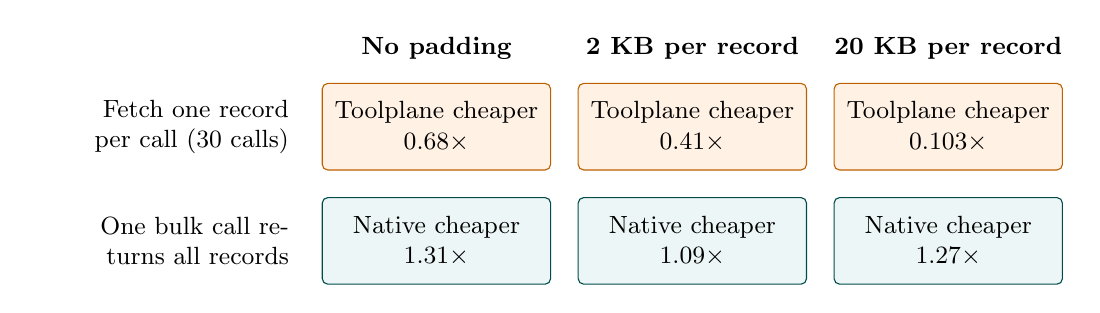
\begin{tikzpicture}[font=\small]
  \node[font=\small\bfseries] at (3.5,2.0) {No padding};
  \node[font=\small\bfseries] at (6.75,2.0) {2 KB per record};
  \node[font=\small\bfseries] at (10.0,2.0) {20 KB per record};
  \node[anchor=east, align=right, text width=3.2cm] at (1.75,1.0) {Fetch one record per call (30 calls)};
  \node[draw=orange!75!black, fill=orange!10, rounded corners=2pt, align=center, minimum width=2.9cm, minimum height=11mm] at (3.5,1.0) {Toolplane cheaper\\0.68$\times$};
  \node[draw=orange!75!black, fill=orange!10, rounded corners=2pt, align=center, minimum width=2.9cm, minimum height=11mm] at (6.75,1.0) {Toolplane cheaper\\0.41$\times$};
  \node[draw=orange!75!black, fill=orange!10, rounded corners=2pt, align=center, minimum width=2.9cm, minimum height=11mm] at (10.0,1.0) {Toolplane cheaper\\0.103$\times$};
  \node[anchor=east, align=right, text width=3.2cm] at (1.75,-0.45) {One bulk call returns all records};
  \node[draw=teal!60!black, fill=teal!7, rounded corners=2pt, align=center, minimum width=2.9cm, minimum height=11mm] at (3.5,-0.45) {Native cheaper\\1.31$\times$};
  \node[draw=teal!60!black, fill=teal!7, rounded corners=2pt, align=center, minimum width=2.9cm, minimum height=11mm] at (6.75,-0.45) {Native cheaper\\1.09$\times$};
  \node[draw=teal!60!black, fill=teal!7, rounded corners=2pt, align=center, minimum width=2.9cm, minimum height=11mm] at (10.0,-0.45) {Native cheaper\\1.27$\times$};
\end{tikzpicture}
\caption{July pilot, payload by API granularity.  Each cell is \toolplane{}
over native median cost (Claude Code, Claude Sonnet 5; Table~\ref{tab:payload},
computed before rounding).  Reading across a row, payload moves the size of
the effect.  Reading down a column, the API's granularity flips its sign.}
\label{fig:payload-matrix}
\end{figure*}


This factorial intervention is the pilot's cleanest result.  Under a
fetch-one API, the native path must emit and observe 30 record calls.  On
median costs, Toolplane costs 0.68$\times$, 0.41$\times$, and 0.103$\times$
native as padding grows.  Give the server one bulk endpoint and the native-client path
wins at every payload: Toolplane costs 1.31$\times$, 1.09$\times$, and
1.27$\times$ native, respectively.  The
observed cost ranges are disjoint in all six comparisons.

The bulk API reduces domain retrieval to one native call.  At 2 and 20~KB,
Claude Code then writes the oversized result to a local file and the agent
processes it with Bash/\texttt{jq} or Python; the full payload does not enter
model context.  The advantage therefore belongs to the complete native-client
path, which performs its own context-decoupled computation, not to avoiding
programming altogether.  The baseline bulk cell remains inline and native
still wins, so result externalization is not the only explanation.

The Toolplane arm is not an oracle implementation: several bulk runs returned or
sampled the large value before aggregating, and the classifier records 19
staged-after-success executions across the 18 Toolplane runs.  We measure agent
behavior, including imperfect program construction.

\finding{Payload size changes how large the effect is; the API's granularity decides
its sign.  With one record per call \toolplane wins at every payload, and with
one bulk call the native path wins at every payload.}



\subsection{Rollback snapshot scaling}

Monty snapshots the complete live namespace before each execution so a timed
out run can be discarded without retaining partial VM mutations.  The
persistence study re-measured this on the shipped Monty 1.1 runtime: seven
back-to-back measurements at each size in one process show snapshot bytes
tracking payload size and median no-op execution at or below 4.72~ms through
10~MB (Table~\ref{tab:snapshot}).

\begin{table*}[t]
\centering
\small
\caption{Persistent-namespace snapshot microbenchmark, Monty 1.1 (recorded with
the persistence study).  ``No-op'' includes the mandatory pre-run
snapshot.}
\label{tab:snapshot}
\begin{tabular}{rrrr}
\toprule
Live payload & Snapshot bytes & Median dump & Median no-op \\
\midrule
1~KB & 2.0~KB & 0.09~ms & 0.30~ms \\
100~KB & 101.0~KB & 0.15~ms & 0.27~ms \\
10~MB & 10.0~MB & 4.10~ms & 4.72~ms \\
\bottomrule
\end{tabular}
\end{table*}

This measures Python-visible allocation and serialization time, not process
RSS.  The 1~KB and 100~KB no-op medians differ by 0.03~ms, below what this
simple microbenchmark can interpret, and the table does not justify
extrapolation to 100~MB namespaces.  The July pilot measured the 0.0.18
in-process runtime (3.48~ms no-op at 10~MB); the two are not comparable, since
the later runtime moves the snapshot behind a worker round trip.




\section{Pilot and Replication Probes}
\label{sec:additional-probes}

The remaining studies are secondary mechanism probes: the July pilot on
Claude Sonnet 5, then four-run October replications.  They explain mechanisms
and failure modes, but they have smaller samples or earlier harness epochs
than the registered studies.  Where a registered cell re-tested a pilot claim,
the subsection says what it found.

\subsection{A fixed intercept meets a growing native-client cost}

The initial experiment compared a single lookup, aggregation over 30 records,
and aggregation over 100 records.  It established the qualitative shape but
also exposed a large, avoidable discovery tax in \toolplane: capability name,
schema, Python binding, and return semantics lived on separate surfaces.
Transcript classification showed agents reading multiple discovery resources
and probing return wrappers before writing a successful program.

We changed the search response to include exact awaitable call shapes and the
plain-value return contract.  A same-day native control reproduced earlier
costs to the cent.  Across nine post-intervention \toolplane runs there were
zero namespace-manifest reads, one search per run, a median of one execution,
and no failed snippets.  Table~\ref{tab:discovery} shows that reducing fixed
discovery work moved the boundary without changing the underlying runtime or
task.

\begin{table}[t]
\centering
\scriptsize
\caption{Discovery intervention: median billed cost over three correct runs
per cell.  The pre-intervention arm used an earlier client version; same-day
direct controls support the cost movement, but this is an engineering
intervention rather than a randomized causal estimate.}
\label{tab:discovery}
\resizebox{\linewidth}{!}{%
\begin{tabular}{lrrr}
\toprule
Task & \toolplane{} before & \toolplane{} after & Native, same day \\
\midrule
Single & \usd{0.26} & \usd{0.18} & \usd{0.14} \\
$N=30$ & \usd{0.24} & \usd{0.18} & \usd{0.20} \\
$N=100$ & \usd{0.28} & \usd{0.18} & \usd{0.33} \\
\bottomrule
\end{tabular}%
}
\end{table}

In this 2.1.205 sweep, the Toolplane arm remains near \usd{0.18} from five to
100 records, whereas native-client cost grows with generated tool calls and
returned records (Table~\ref{tab:crossover}).  Native registration is clearly
cheaper below 10 records.  At 20 and 30 records the observed ranges overlap,
so the arm difference is unresolved at three repetitions.  At 100 records,
Toolplane is approximately 45\% cheaper in this sweep, with disjoint observed
ranges.

\begin{table}[t]
\centering
\scriptsize
\caption{Earlier 2.1.205 interaction sweep after the discovery intervention.
Values are medians; each cell has three correct runs.  A dagger marks
overlapping observed ranges between arms, not equivalence.}
\label{tab:crossover}
\resizebox{\linewidth}{!}{%
\begin{tabular}{lrrrrr}
\toprule
Records touched & 5 & 10 & 20 & 30 & 100 \\
\midrule
Native & \textbf{\usd{0.13}} & \textbf{\usd{0.14}} & \usd{0.18}$^{\dagger}$ & \usd{0.20}$^{\dagger}$ & \usd{0.33} \\
\toolplane & \usd{0.18} & \usd{0.17} & \usd{0.18}$^{\dagger}$ & \usd{0.18}$^{\dagger}$ & \textbf{\usd{0.18}} \\
\bottomrule
\end{tabular}%
}
\end{table}

A later hardened 2.1.207 fetch-one cell at $N=30$ does not reproduce the
unresolved result: native cost is \usd{0.171} [\usd{0.158}, \usd{0.191}], while
Toolplane costs \usd{0.116} [\usd{0.100}, \usd{0.142}], a 32.3\% reduction
with disjoint observed ranges.  Client version, harness epoch, and task details
therefore prevent us from localizing one current crossover point by pooling
the two studies.

The registered Claude Haiku 5.5 matrix confirms the direction at both ends
(1.11--1.13$\times$ at one and five records, 0.50$\times$ at 100) and places the
crossing between 5 and 20 records, but it tested only the ends; no study here
localizes a single crossover point across epochs.

\finding{\toolplane costs more to start and less per record.  The registered result
is a loss on small tasks and a gain on large fine-grained ones; no study here
fixes a single crossover point.}

\subsection{Why round trips do not explain the win}

The pilot saw the mechanism first, in request IDs;
Table~\ref{tab:tokens} later confirmed it in token classes.  This subsection
keeps only the pilot's own evidence.
Native-client Claude Code grouped many independent tool calls into a small number of
model responses.  At $N=100$, the native arm produced 103 tool invocations but not 103
model requests.  Conversely, the Toolplane arm required search, code execution,
and answer-generation requests.  Exact request IDs in the clean
post-intervention traces give median request counts of 4 versus 6 at $N=30$
and 5 versus 6 at $N=100$ for native and Toolplane respectively.  The Toolplane arm
therefore makes more requests and still wins at $N=100$.

The scaling term is instead model-generated tool syntax and model-visible
results.  Every native \texttt{get\_order} requires an output-token tool block;
every returned record becomes conversation material unless the client
externalizes it.  At $N=100$, the native arm generated roughly 7.5K output tokens for a
three-line aggregate.  The Toolplane arm generated one loop and returned only the
aggregate, leaving intermediate records in the sandbox.  Parallel scheduling
reduces native wall time but does not remove generated syntax or conversation
growth.

The later payload experiment records exact request counts under the hardened
harness.  At 20~KB/fetch-one, the native arm batches 30 record fetches into a median of
four model requests and 32 tool uses; the Toolplane arm uses a median of five model
requests and four tool uses, yet costs 0.10$\times$ native.  This cleanly separates
request batching from payload isolation.  The registered matrix shows the
same split in its token classes (Table~\ref{tab:tokens}): generated output at
small payloads, uncached input at large ones.

\finding{Tool calls and model requests are different counts.  Because the client
batches calls, \toolplane's advantage is less generated output and less
intermediate data in context, not fewer round trips.}



\subsection{A templated chain handled stepwise}
\label{sec:chain}

The chain task follows a four-hop thread.  Each fetched note names a true next
order and a decoy, prompting the agent to interpret the current result before
choosing the next call.  Both arms are correct in all three runs, but native
costs \usd{0.17} versus \usd{0.24} for Toolplane: the latter is 38\% costlier
on unrounded medians, with wall medians of 22.9 versus 27.9 seconds and
disjoint observed ranges.

Every code run used five separate \texttt{execute\_code} calls---one per node,
with no execution errors.  The agent did not turn the whole chain into one
program; it reproduced native stepwise tool use inside a heavier interface.
The fixture is template-generated and can be traversed by a hand-written
regex, so this experiment measures the strategy agents selected for an
adaptive-looking task, not the theoretical impossibility of code batching.
The 38\% gap (1.36$\times$ on cost of pass) belongs to this July point: on
cost of pass the same templated chain measured 1.07$\times$ in the October
re-run on Sonnet 5, 1.05$\times$ in four runs on Sonnet 5.5, and 1.12$\times$
in the registered Haiku 5.5 matrix.  A prose chain built to resist
heuristic shortcuts (Section~\ref{sec:october}) gave the same behavior.

\finding{On the templated chain the agent made one decision per fetched note, so the
\toolplane arm did the same stepwise work as the native arm and paid for one
extra execution per step.}

\subsection{Tool latency and concurrency}
\label{sec:latency}

We added 100~ms of server-side latency to each of the 31 calls in the
$N=30$ loop.  On the original await-triggered runtime, external calls
dispatched only when awaited, so the recorded snippets' 31 sequential awaits
added a deterministic 3.1 seconds to that execution path.  End-to-end
Toolplane wall medians moved from 20.9 to 23.6 seconds with overlapping
ranges (unresolved at three repetitions), while native wall showed no
corresponding increase, consistent with Claude Code batching independent
calls.  Toolplane retained the observed wall-time lead at 100~ms in that
epoch.

The later eager-dispatch runtime changed the mechanism: external calls
dispatch when invoked, so firing calls before awaiting them overlaps the
latency --- at this fixture's shape, 30 calls at 100~ms complete in
0.24~seconds through the mediated path versus 3.3~seconds serial (measured
host-side, without a model).  Re-running the cell on the new runtime with
concurrency guidance present in the search footer, namespace manifest, and
skill documentation produced wall parity with the native arm (medians 30.3
versus 28.4~seconds, ranges overlapping): the runtime could overlap, but all
five recorded snippets still awaited serially inside the loop body.  Adding
the fan-out idiom to the \texttt{execute\_code} tool description --- the one
surface the model always reads before writing --- flipped adoption from 0/5
to 4/4 snippets on the same cell and client version, and flipped the wall
result with it: Toolplane medians of 22.8 versus 28.4~seconds for the native
arm, with disjoint ranges, at 29\% lower cost (three repetitions per arm,
counterbalanced; the native reference rows come from the same-evening control
matrix).

\finding{A runtime that can run calls concurrently helped only once the agent was
shown the idiom in the tool description it reads first.  The registered
re-test left the wall-time difference unresolved.}



\subsection{Deferred loading shrinks the unused-schema tax}

A common argument for code mode is that a single facade prevents dozens of
tool schemas from occupying every prompt.  We varied configured MCP servers
from 1 to 5 to 15, reaching 84 capabilities at the largest setting.  At
$N=30$, the native-minus-Toolplane cost is non-monotone: native/Toolplane medians are
\usd{0.20}/\usd{0.22}, \usd{0.20}/\usd{0.18}, and
\usd{0.23}/\usd{0.23} at $M=1,5,15$.  With three runs per cell, this is not a
registry-size trend.

The trace mechanism is stronger than the noisy medians.  The committed $M=15$
init-event probe lists no loaded MCP tools; Claude Code exposes deferred stubs
instead.  All 18 native-arm rows across $M$ make one client-level
\texttt{ToolSearch}, load only the order tools, and select no distractor; all
36 runs are correct.  At $M=15$, none of the 82 distractor schemas is present
in the probed native context.  Two $M=15$ native runs include unrelated Bash
exploration, which explains much of their residual cost increase.  The
distractors are semantically distant, so this experiment does not test
near-miss retrieval.

The registered Haiku 5.5 matrix measured the native arm at $M=15$ against
$M=1$ with eight runs each: +3\%, with an interval inside the $\pm$10\% margin
but excluding zero (H8, Section~\ref{sec:confirm}).  The tax is small, not
absent.

\finding{With deferred loading, fifteen configured servers cost the native arm about
3\% more than one.  The number of schemas configured is not the number the
model sees.}

\subsection{Hybrid routing is task- and scale-dependent}

We tested a hybrid facade that re-exported capabilities as native MCP tools
alongside search and execution.  At $M=1$ and two repetitions, the model routed
single lookup and chain tasks to native tools and loops to code in every run,
but economics remained task-dependent.  Native/facade/hybrid medians were
\usd{0.128}/\usd{0.148}/\usd{0.141} for single,
\usd{0.205}/\usd{0.181}/\usd{0.155} at $N=30$,
\usd{0.329}/\usd{0.180}/\usd{0.154} at $N=100$, and
\usd{0.169}/\usd{0.182}/\usd{0.233} for the chain.  Hybrid wins the loops but
is worst on the chain.  Neither code path invokes Toolplane's capability-search
meta-tool (both may still use client-level
\texttt{ToolSearch}); hybrid succeeds with one execution versus two or three
under the pure facade.

At $M=15$, all-capability hybrid exposes 87 tools rather than the facade's
three.  On the two measured lookup/chain tasks, it is the most expensive
arm: \usd{0.26} for single and \usd{0.28} for chain, versus native's
\usd{0.13} and \usd{0.19}.  These are two-repetition results, and loops were
not run at $M=15$; they demonstrate a failure mode, not a characterized scale
curve.  Loading the facade namespace also loaded 84 re-exported schemas,
rebuilding the context surface the facade was intended to hide.

Selective re-export, at two repetitions per task, reduces the visible surface
from 87 to five tools but does not consistently improve cost: it improves the
single task relative to all-capability hybrid and is slightly worse on the
chain.  Follow-up name/description A/Bs are exploratory and are summarized in
Appendix~\ref{app:naming-ab}; they show no detectable repair of
client-mediated retrieval in the two tested domains.

\finding{Whether an agent routes a task to a native tool or to code is its own
behavior, not something the server sets.  Re-exporting a few tools helped at
small scale; re-exporting a whole registry did not, and renaming tools did
not repair retrieval.}



\subsection{October replications}
\label{sec:october}

Three four-run studies preceded the registered matrix.  Each is reported in
full in \texttt{docs/code-mode-benchmark.md}.

\paragraph{The shipped runtime, and a new failure.}  Re-running seven pilot
cells on \toolplane 0.5.0 (Monty 1.1) with Claude Sonnet 5 and Claude Code
2.1.293, 24 of 24 \toolplane runs that reached the backend were correct.  The
discovery turn was gone: no run called \toolplane's capability search, because
the facade's tool descriptions now carry call shapes, and \toolplane's wall
time roughly halved at every task size.  The re-run also found the study's
first behavioral failure: 4 of 28 \toolplane runs abstained, answering in one
turn that they had no access to order data without calling any tool.  None of
21 July runs and none of 28 same-day native runs abstained.  A follow-up
registered on the issue tracker found no abstention on the newer models (0 of
60 Claude Haiku 5.5 runs and 0 of 40 Claude Sonnet 5.5 runs), and the
confirmation matrix later recorded none in 232 Haiku runs.  The follow-up ran
only the 30-record cell, where Sonnet 5 itself had not abstained, so the
trigger was never reproduced; it is recorded as a Claude Sonnet 5 behavior with
that caveat.

\paragraph{A second client.}  On Codex CLI 0.160.0, whether the boundary
exists depends on the model, because Codex gates its own built-in code mode per
model.  With gpt-5.5, which makes ordinary per-tool calls, the Claude Code
pattern reappears: a single lookup uses 2.4 times the input, while a 30-record
loop uses 25\% less input and 76\% less output, and a 100-record loop 92\% less
output.  With gpt-6.1-sol, which reaches MCP tools only through Codex's own
JavaScript code mode, input differs by 5\% or less, walls overlap, and output
is 8--24\% higher for \toolplane on the small tasks: code mode calling code
mode leaves little to gain and costs little.  Codex on a subscription
plan reports tokens, not dollars, and these are four-run cells.

\paragraph{A code-resistant chain and a CLI + MCP join.}  On Claude Sonnet 5.5,
a prose chain whose notes identify the next order only by meaning (five
heuristic shortcuts, pinned in tests, all walk to the wrong order) gave the same
result as the templated chain: every run in both arms walked hop by hop, at
1.08$\times$ native cost.  One shortcut stays open --- fetch all notes in one
program and read them --- and no agent took it.  A join task whose refund list
lives in git history and whose amounts live behind MCP measured
1.22$\times$ native with a shell available --- most likely because
\toolplane runs explored the repository through Bash first, though they also
made one capability search each --- and 0.94$\times$ with the shell removed and
git reached through \toolplane's CLI binding.  The registered Haiku 5.5
re-test of the same join is in Section~\ref{sec:confirm} (H7a and H7b).

\section{A Conditional Empirical Envelope}
\label{sec:envelope}

The measurements sort tasks by what the model contributes at each step.  Where
it only carries values between tools, a program is cheaper once there are
enough of them.  Where the agent decides step by step, or a single call
already returns everything, there is little glue to remove and the fixed
cost of the program is not repaid.  The measurements support a decision envelope for the
tested system, not a predictive law.  Table~\ref{tab:decision} states the observed direction and the
mechanism that must hold for it to transfer; Figure~\ref{fig:decision-flow}
summarizes the same logic as a checklist.

\begin{table*}[t]
\centering
\small
\caption{Observed decision envelope.  Registered ratios are Claude Haiku 5.5
cost of pass, \toolplane over native, except the session row (Claude Sonnet
5.5).  Directions should be tested before use as a routing policy.}
\label{tab:decision}
\begin{tabular}{>{\raggedright\arraybackslash}p{0.27\linewidth}>{\raggedright\arraybackslash}p{0.18\linewidth}>{\raggedright\arraybackslash}p{0.45\linewidth}}
\toprule
Condition & Observed preference & Mechanism \\
\midrule
Single lookup or about five fine-grained calls & Native (registered:
1.11--1.13$\times$) & Fixed search/code overhead cannot amortize \\
20--30 small fetch-one records & Toolplane (registered at 30:
0.82$\times$) & 20 was run but not tested (0.93$\times$); the July Sonnet 5
ranges at 20 and 30 overlapped \\
Many fine-grained fetch-one calls, especially with large model-visible results
& Toolplane (registered: 0.50$\times$ at 100; 0.020$\times$ at 20~KB) &
Generated call syntax and intermediate payload stay outside model context \\
Native bulk endpoint & Native (registered: 1.05--1.31$\times$) & One domain
call removes fine-grained composition; large results may enter the client's own
file/code path \\
Chain handled stepwise, templated or prose & Native (registered: 1.12$\times$)
& Toolplane adds one execution envelope per agent-selected stage \\
Slow independent calls, serial sandbox awaits & Native pressure (pilot) &
Client batches native calls while the runtime pays approximately $K\ell$ \\
Slow independent calls, fan-out idiom taught & Toolplane on cost; wall time
unresolved (registered) & Eager dispatch collapses the sandbox path to about
$\ell$; the pilot's wall-time win did not replicate with an interval \\
Large, semantically distant registry with deferred loading & Small native
schema tax (registered: +3\% at $M=15$) & Unused schemas mostly stay out of
model context \\
Related queries over already loaded data & Session total: Toolplane
(registered: $-$40\%); each reuse turn: native (+35\%) & The saving is the
load; every reuse turn needs an extra executor request \\
Client that already runs its own code mode & Neither (Codex gpt-6.1-sol, four
runs) & Code mode calling code mode leaves little to save \\
\bottomrule
\end{tabular}
\end{table*}

\begin{figure*}[t]
\centering
\resizebox{0.82\textwidth}{!}{%
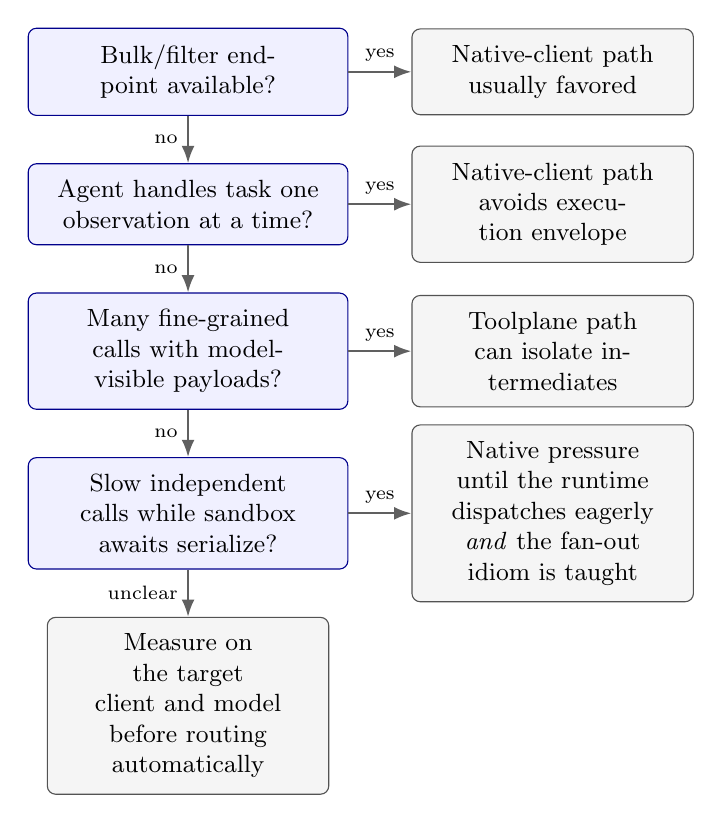
\begin{tikzpicture}[node distance=6mm and 8mm]
  \node[questionbox] (bulk) {Bulk/filter endpoint available?};
  \node[resultbox, right=of bulk] (nativebulk) {Native-client path\\ usually favored};
  \node[questionbox, below=of bulk] (stepwise) {Agent handles task one observation at a time?};
  \node[resultbox, right=of stepwise] (nativestep) {Native-client path\\ avoids execution envelope};
  \node[questionbox, below=of stepwise] (fine) {Many fine-grained calls with model-visible payloads?};
  \node[resultbox, right=of fine] (codewin) {Toolplane path\\ can isolate intermediates};
  \node[questionbox, below=of fine] (latency) {Slow independent calls while sandbox awaits serialize?};
  \node[resultbox, right=of latency] (nativepressure) {Native pressure until the runtime dispatches eagerly \emph{and} the fan-out idiom is taught};
  \node[resultbox, below=of latency] (measure) {Measure on the target\\ client and model\\ before routing automatically};

  \draw[flowarrow] (bulk) -- node[above, font=\scriptsize] {yes} (nativebulk);
  \draw[flowarrow] (bulk) -- node[left, font=\scriptsize] {no} (stepwise);
  \draw[flowarrow] (stepwise) -- node[above, font=\scriptsize] {yes} (nativestep);
  \draw[flowarrow] (stepwise) -- node[left, font=\scriptsize] {no} (fine);
  \draw[flowarrow] (fine) -- node[above, font=\scriptsize] {yes} (codewin);
  \draw[flowarrow] (fine) -- node[left, font=\scriptsize] {no} (latency);
  \draw[flowarrow] (latency) -- node[above, font=\scriptsize] {yes} (nativepressure);
  \draw[flowarrow] (latency) -- node[left, font=\scriptsize] {unclear} (measure);
\end{tikzpicture}%
}
\caption{Checklist form of the observed envelope.  The diagram is not an
automatic router: each branch encodes a mechanism observed in this
Claude Code/Toolplane case study (registered on Claude Haiku 5.5) and requires validation before transfer
to another client, model, runtime, or workload.}
\label{fig:decision-flow}
\end{figure*}

The envelope can be read as a sequence of questions:

\begin{enumerate}
  \item Does the server expose the measured bulk retrieval operation?  The
  native-client path avoids Toolplane's programmable layer; at large payloads
  it may still perform context-decoupled work through its own file/code path.
  \item Does the agent handle the task one observation at a time?  In the
  measured templated and prose chains, native registration avoids repeated
  execution envelopes.  The prose chain was built so that no heuristic we
  tried can shortcut it, though one program that fetches every note and hands
  them all to the model remains possible; no agent tried it.
  \item Otherwise, are there many fine-grained calls with model-visible
  intermediate results?  Toolplane can prevent generated call syntax and
  payload ingress from scaling with the task.
  \item Are calls slow and independent?  The answer depends on whether the
  code runtime can fan them out as effectively as the client --- and on
  whether the fan-out idiom is taught where the agent reads it.
\end{enumerate}

A task-specific server-side filter or aggregate should further favor the
native path under the cost model, but that branch is a prediction: this study
measures bulk retrieval, not server-side answer computation.

Most of this envelope's directions were pre-registered and confirmed on Claude
Haiku 5.5, but on the same order-store domain on which the pilot discovered
them.  Predicting winners on held-out domains remains untested, so
``envelope'' means a synthesis of controlled observations, not validated
automatic routing or a claim of optimal interface selection.

\section{Related Work}
\label{sec:related}

\paragraph{Executable actions and context-decoupled agents.}
CodeAct replaces constrained JSON/text actions with executable Python and
reports improved task success across models \cite{wang2024codeact}; DynaSaur
lets agents create, compose, and reuse programmatic actions dynamically
\cite{nguyen2025dynasaur}.  Felendler et al. provide the closest direct MCP
architectural comparison: they formalize context-coupled and code-execution
MCP, measure tokens, latency, turns, and task quality across servers and
models, and develop a security taxonomy \cite{felendler2026mcp}.  LOCA-bench
independently controls environment-driven context growth while holding task
semantics fixed and evaluates programmatic tool calling among several context
management strategies \cite{zeng2026loca}.  CoDA isolates planner and executor
contexts, while ATLAS combines progressive MCP loading with programmatic
orchestration for learned small-model agents
\cite{liu2026coda,gupta2026atlas}.  These works establish the representational
and context-management value of executable or isolated action paths.  We
neither claim the first direct-versus-code comparison nor contribute a
security taxonomy.  Our narrower contribution is billed-cost and trace-level
localization across interaction, payload, granularity, discovery, latency,
and persistent-session axes in one production client.

\paragraph{Production systems.}
Anthropic reports both a roughly 38\% billed-input reduction on a 75-tool
project-management benchmark and roughly 8\% higher cost with unchanged scores
on sequential $\tau^2$-bench tasks making one or two calls per turn
\cite{anthropic2026ptc}.  Cloudflare reports large static schema-token
reductions for a code-mode API facade
\cite{cloudflare2026codemode}, following its earlier proposal to convert MCP
tools into a typed API executed in a sandbox \cite{cloudflare2025codemode};
Anthropic's engineering reports motivate the same context-isolation pattern
\cite{anthropic2025codemcp,anthropic2025advancedtools}.  The goose agent
ships an open-source code mode, and its maintainers report 30\% fewer tokens
on one task while noting that for simple single-tool tasks the overhead is
not worth it \cite{goose2026codemode}.  Codex CLI ships its
own JavaScript code mode and enables it per model; in our replication, models
with it routed every MCP call through code, while gpt-5.5 made plain tool
calls (Section~\ref{sec:october}).  Workload-dependent
gains and losses are therefore already publicly documented.  Our contribution
is not the first reported reversal; it is an independently reproducible,
multi-axis measurement with committed raw artifacts and explicit
counterexamples.

\paragraph{Tool retrieval and dynamic catalogs.}
ToolLLM and AnyTool study selection from very large API collections
\cite{qin2023toolllm,du2024anytool}.  MCP-Zero and SING retrieve capabilities
from evolving model intentions while minimizing schema exposure
\cite{fei2025mcpzero,xiao2026sing}; MemTool manages tool context across long
conversations \cite{lumer2025memtool}.  CodeNav lets agents search and import
code rather than consume registered tool descriptions
\cite{gupta2024codenav}.  These works primarily optimize recall, success, or
schema tokens.  Among the works we reviewed, none reports discovery as
incremental production-client model requests and prices those requests in a
controlled direct-versus-code comparison.  Our registry and hybrid results
also show why catalog size alone is an insufficient independent variable when
the client defers loading.

\paragraph{Agent interfaces, caching, concurrency, and economic evaluation.}
SWE-agent demonstrates that agent-computer interface design materially changes
model behavior \cite{yang2024sweagent}; our object is a specific economic
interface boundary rather than the first interface-design result.  Prompt
caching can reduce agent cost and latency substantially
\cite{lumer2026cache}, making it essential to price cache reads rather than
compare raw context sizes.  Asynchronous function-calling work studies latency
benefits from parallel execution \cite{gim2024asynclm}, while TPS-Bench and
BFCL evaluate planning, scheduling, parallel calls, and tool-use quality
\cite{xu2025tpsbench,patil2025bfcl}.  These evaluations treat parallel
execution as a capability to be measured.  Our latency A/B isolates a further
variable they do not price: whether the model actually writes the concurrent
idiom.  A verified runtime capability produced no measured benefit until the
idiom moved into the executor's tool description
(Section~\ref{sec:latency}) --- an adoption effect in the spirit of
SWE-agent's interface result, at the granularity of a single description
sentence.  Cost-of-Pass and AI Agents That Matter
argue for economically grounded evaluation rather than accuracy-only rankings
\cite{erol2026costofpass,kapoor2025agentsmatter}.  We apply that principle to
the interface crossover; we do not claim the first cost-aware agent benchmark.

\section{Threats to Validity}
\label{sec:limitations}

\paragraph{Few clients and models, one code-mode implementation.}
Claude Code's ToolSearch, native batching, built-ins, prompt caching, and
result-file externalization are central causal actors, and each model's routing
and program-writing behavior is inseparable from the client treatment.  The
registered evidence covers Claude Haiku 5.5 (cost envelope) and Claude Sonnet
5.5 (sessions) in one Claude Code version.  Codex with two models is a
four-run replication reporting tokens rather than dollars.  Claude Sonnet 5
abstained in October but not in July under the same model string, while the
runtime, the facade's descriptions, and the client had all changed, so a
behavior can appear without any change on the measured side of the
interface.  An independent code-mode implementation is untested.

\paragraph{Synthetic and narrow domains.}
Most economic tasks use formula-generated order records.  This gives exact
correctness and controllable payloads, but aggregation naturally favors code
and does not represent a workload distribution.  The 2~KB and 20~KB payload
levels are unused synthetic detail strings, not samples from a real domain;
they isolate payload ingress rather than payload semantics.  The shipment
domain is used only to challenge a discovery naming hypothesis.  The
strongest further validation would add genuinely different document/search and
operational API domains, including quality-sensitive tasks where both arms can
fail.

\paragraph{Small samples and multiplicity.}  The registered studies use eight
runs per arm (four in the 20~KB cells) with bootstrap intervals; pilot cells
have two to four, and hybrid cells often two.  The pilot evolved through many
interventions and carries multiple-comparison and researcher-degrees-of-freedom
risk; the registrations exist to bound it.  The confirmation matrix tests 22
rows without a multiplicity correction, and some of its cells are nearly
deterministic, so a single outlier can decide an interval.  Two procedural
lessons are recorded for later registrations: run one discarded warm-up per
block, because the first run after a cache expiry pays cache creation, and
test equivalence margins first.

\paragraph{Native baseline and API design.}
The bulk intervention repairs an important weak-baseline concern, but
server-side filters and aggregates remain unmeasured.  A server-side operation
that returns exactly the requested answer should usually favor native tools;
testing it would measure the boundary rather than overturn the model.  Large
bulk results also trigger a client-specific file/Bash path.  Consequently,
those cells compare Claude Code's native MCP + result-file + Bash/Python path
with Toolplane-mediated execution; they do not isolate a pure ``direct,
no-code'' paradigm.

\paragraph{Cost and correctness.}
Most cells are fully correct, which makes cost comparison clean but says little
about quality.  Three failures are the exception, and each is a model behavior
the cost model does not contain: Claude Sonnet 5 abstaining behind the generic
facade (4/28), Claude Haiku 5.5 degenerating after 30 native fetches of 2~KB
records (0/8), and Claude Haiku 5.5 never searching for the facade when a shell
was available (2/8).  Cost of pass prices them in, so two registered verdicts
hold through them; we report those as correctness results.  Tasks where both
interfaces can fail on quality remain untested.

\paragraph{Implementation versus paradigm.}
Fixed discovery cost, runtime syntax support, and agent-authored retry behavior
are properties of the measured \toolplane version.  The latency cells further
show results moving with runtime dispatch semantics (await-triggered versus eager)
and with where concurrency teaching is placed; other code-mode systems may
search, batch, sandbox, expose types, or document concurrency differently.
Conversely, native performance depends on whether the client defers tools and
externalizes large results.  We distinguish these mechanisms rather than
attributing all observations to an abstract paradigm.

\paragraph{Temporal prices and latency.}
Dollar values depend on provider pricing, caching policy, client version, and
run date.  Raw token classes exist for all rows; exact request IDs and complete
transcripts exist for later harness epochs.  These permit partial repricing and
trace reanalysis.  Wall-clock variance includes remote model service behavior;
cross-version wall times are not compared.

\paragraph{Security is out of scope.}
Code execution expands the attack surface and changes auditability.  The
experimental runtime is sandboxed and capabilities traverse host policy and
audit gates, but this paper does not evaluate adversarial safety.  Felendler et
al. provide a dedicated taxonomy and defense analysis
\cite{felendler2026mcp}.  Performance evidence must not be read as a security
endorsement.

\section{Reproducibility and Research Practice}

The repository publishes the benchmark driver, deterministic fixtures,
validators, and raw JSON for all reported runs.  For matrices on the hardened harness
it also publishes complete redacted transcripts, classifiers, exact model
request accounting, and frozen-code provenance.  Later rows stamp the built
wheel, fixture set, base harness, and experiment-specific harness hashes.  The
paper's evidence map names the primary artifact for each table and marks weaker
epochs.

Both October studies were pre-registered: the plan, hypotheses, decision rule
and analysis script were committed before any data, and the results documents
report every verdict, including the reversed and unresolved ones, with
independent recomputation from the raw rows.

We also retain failures of the research process.  A contaminated paid matrix
is named and excluded rather than deleted.  Negative product hypotheses---the
templated chain, all-capability hybrid, selective re-export, naming intervention,
and compounding-session story---are reported alongside wins.  Post-hoc changes
are explicit: one correctness validator was semantically rescored without
changing answers, and longitudinal per-turn token fields were replaced from
verbatim result events after an accounting error.  The shipment naming runs'
dirty, not-fully-hash-covered harness provenance is retained rather than
presented as clean.  None of these corrections changes the primary
tables in this paper.

This transparency does not substitute for independent replication, but it
makes disagreement testable.  The artifact is MIT-licensed.  It does not yet
include a machine-readable pricing schedule, so re-pricing the token classes
at other rates is left to the reader.

\section{Conclusion}

What separates the two interfaces is what the model does at each step: carry
values, or decide.  Native-client MCP orchestration and Toolplane-mediated
execution are not ordered by a single notion of task complexity.  In the measured system,
Toolplane pays a fixed discovery and program-generation cost, then avoids
model-generated per-call syntax and model-visible intermediate payload.  A
pre-registered matrix on Claude Haiku 5.5 confirms the shape the July pilot
found: native registration wins a single lookup and a five-record loop by
11--13\%; Toolplane halves cost at 100 fine-grained calls and is 50 times
cheaper when those calls return 20~KB records.  A native bulk API reverses
the winner, and agents walk chains step by step, so the native path wins
those too, even on a chain written to resist shortcuts.  Request counts barely
differ between arms: the advantage is output tokens at small payloads and
uncached input at large ones.  Client mechanisms erase textbook arguments on
both sides: deferred loading leaves only a small schema tax, while result
externalization gives the native arm its own context-decoupled file/code path.
Slow calls make the boundary second-order: the pilot's wall-time win needed both
eager dispatch and a taught fan-out idiom, and the registered re-test left it
unresolved.

The persistence study sharpens the data-ingress mechanism.  On Claude Sonnet
5.5 a Toolplane session lowers five-turn cost by 40\% and peak context by 38\%,
but the gap opens on the initial load; each reuse turn then costs about a third
more than native conversation reuse, because the session needs an executor
call before it can answer.  Against a sessions-off Toolplane arm the live
session is 7\% cheaper, but that arm refetched inside the sandbox instead of
using the result store, so the store's economic contribution is not isolated.

The practical conclusion is conditional, and it follows from what the model
contributes at each step.  Where the model only carries values between tools,
it is glue, and in the measured system that glue cost less in a program:
prefer Toolplane when many fine-grained calls expose intermediate results,
especially large ones, and when the client does not already run its own code
mode.  Where there is little to carry, or the agent decides step by step,
keep the model in the loop: prefer the native-client path for a handful of
calls, when a sufficient bulk operation exists, or when agents handle a chain
stepwise.  ``Use the model for judgment, not for glue'' is a mnemonic for
these measurements, on one domain and a small set of clients and models.  It
is not a decision rule, and not a law.  Treat discovery, client behavior, and runtime
concurrency as first-class parts of the system: the study's three failures are
model behaviors at the interface, not runtime errors.  More broadly, Toolplane
is useful when a small programmable surface over MCP, CLI, and host/Python
capabilities is worth an extra execution layer; this paper identifies
conditions under which that trade-off is economically visible.  Held-out
domains and further clients are the next step from this case study to a
general result.

\bibliographystyle{plain}
\bibliography{references}

\onecolumn
\appendix
\section*{Appendix}
\addcontentsline{toc}{section}{Appendix}
\section{Evidence Tier Map}
\label{app:evidence-tiers}

\begin{table}[H]
\centering
\small
\caption{Evidence tiers used for interpretation.}
\label{tab:evidence-tiers}
\begin{tabular}{p{0.18\linewidth}p{0.34\linewidth}p{0.38\linewidth}}
\toprule
Tier & Evidence & Role in the paper \\
\midrule
Primary & Registered confirmation matrix (Claude Haiku 5.5); registered
persistence study (Claude Sonnet 5.5) & Anchor the cost, context, and session
conclusions \\
Secondary & July payload $\times$ granularity and longitudinal pilot; July
crossover, templated chain, latency and latency-adoption A/B, registry size,
hybrid routing; October four-run replications (runtime re-run, Codex, prose
chain, CLI join) &
Mechanism probes and replications; useful for the envelope but not population
estimates \\
Exploratory & Naming/description A/Bs, pre-hardening pilots, the confirmation
matrix's two-run Sonnet 5.5 slice, and corrected historical rows & Hypothesis generation and provenance, not standalone support
for headline claims \\
\bottomrule
\end{tabular}
\end{table}

\section{Primary Artifact Map}
\label{app:artifacts}

\begin{table}[H]
\centering
\small
\caption{Committed source artifacts for the manuscript's principal results.}
\begin{tabular}{>{\raggedright\arraybackslash}p{0.34\linewidth}>{\raggedright\arraybackslash}p{0.56\linewidth}}
\toprule
Result & Artifact \\
\midrule
Original single/$N=30$ and $N=100$ &
\texttt{run-20260708-123900.json}; \texttt{run-20260708-124546.json} \\
Registry $M=1/5/15$ & \texttt{run-20260709-114215.json} \\
Discovery intervention & \texttt{run-20260709-221840.json} and transcripts \\
Crossover, templated chain, latency & \texttt{run-20260709-235016.json} and transcripts \\
Latency control and adoption A/B & \texttt{run-20260719-023232.json};
\texttt{run-20260719-025053.json} and nine transcripts \\
Hybrid and curated hybrid & \texttt{run-20260711-001559.json};
\texttt{run-20260711-002646.json}; \texttt{run-20260711-014100.json} \\
Naming/description A/B & \texttt{run-20260712-014825.json};
\texttt{run-20260712-015009.json}; \texttt{run-20260712-015759.json};
\texttt{run-20260712-100935.json}; \texttt{run-20260712-101102.json} \\
Payload $\times$ granularity & \texttt{run-20260713-040737.json} and 36 transcripts \\
Longitudinal pilot &
\texttt{longitudinal-20260713-095957.json} and eight transcripts \\
Confirmation matrix &
\texttt{run-20261010-115818.json} through \texttt{run-20261010-142344.json}
(eight files) and transcripts; \texttt{PREREG-confirmation-2026-10.md};
\texttt{RESULTS-confirmation-2026-10.md} \\
October runtime re-run; abstention follow-up & \texttt{run-20261008-012307.json};
\texttt{run-20261008-082359.json}; \texttt{run-20261008-091632.json} \\
Codex replication & \texttt{run-20261008-202709.json};
\texttt{run-20261008-203351.json} \\
Prose chain; CLI + MCP join & \texttt{run-20261009-131413.json};
\texttt{run-20261009-132058.json} \\
Persistence study, Sonnet 5.5 slice, Monty 1.1 snapshots &
\texttt{longitudinal-20261010-191310.json} and 24 transcripts;
\texttt{run-20261010-192444.json} and 32 transcripts;
\texttt{PREREG-persistence-2026-10.md}; \texttt{RESULTS-persistence-2026-10.md} \\
\bottomrule
\end{tabular}
\end{table}


\section{Naming and Description A/B Details}
\label{app:naming-ab}

The follow-up retrieval A/Bs were exploratory because model-generated search
queries vary by arm and the shipment rows retain dirty, not-fully-hash-covered
harness provenance.  On orders ($n=11$ per arm), first-search hits are 11/11
native, 4/11 control, 6/11 name, and 4/11 description; name versus control has
Fisher $p=.67$.  On shipments ($n=9$), first-search hits are 9/9 native, 2/9
control, 3/9 name, and 3/9 description, with $p=1.0$.  The narrow conclusion is
that server-side name or description changes did not detectably repair
client-mediated retrieval in these two domains.  The client-set server
qualifier and competition with built-in tools remain plausible mechanisms, not
isolated causes.

\section{Longitudinal Correction and Reset Revalidation}
\label{app:reset}

\paragraph{Disclosed exceptions.}  Several exceptions are retained and disclosed.  One discovery-tax matrix was
contaminated by a mid-run facade change; it is committed under a
\texttt{mixed-facade} name and excluded.  An early correctness validator was
semantically rescored from committed answers without changing answers or
usage.  The shipment naming runs recorded \texttt{git\_dirty=true}; their wheel
is anchored and fixture hashes match the subsequently committed bytes, but
the then-uncommitted \texttt{bench/run.py} was not hash-covered.  Finally, the
longitudinal harness initially differenced token usage fields that were
already per-turn.  Those four fields were deterministically replaced from the
committed result events; normalized comparison showed no change to cost,
context, answers, fixture calls, or published table values.  No paid run was
repeated for these corrections.

\paragraph{The longitudinal correction.}
The recorded longitudinal result events expose per-turn usage, but the first
analysis treated those counters as cumulative and subtracted adjacent turns.
This produced negative values in four token fields.  The committed artifact
replaces only those fields from each transcript's verbatim result event.  A
normalized before/after comparison established that billed cost, peak context,
answers, correctness, request counts, and fixture calls did not change.  The
economic analysis in Section~\ref{sec:sessions} uses billed cost and
request-context values unaffected by the correction.

The reset predicate was also strengthened after the paid run.  The final
predicate requires a sole, zero-argument reset in the first execute-bearing
assistant event, a matching non-error tool result, and calculation in a later
assistant event.  It independently revalidates all four committed reset-turn
transcripts of the pilot.  The reset turn is contract evidence and is excluded
from the five-turn economic comparison.

In the pre-registered study the same predicate credited 6 of 8 \toolplane
resets.  The other two transcripts show \texttt{return await reset\_session()}
as the sole statement of its own execution, followed by a full refetch and a
correct answer; the predicate accepted only the bare-statement form.  Reset is
reported, not tested, so no verdict depends on it, and the registered figures
stand as recorded.  The predicate was fixed afterwards for future runs; replayed
over these transcripts it credits 8 of 8.

\end{document}
